% Ce fichier main.tex est le fichier principal \`{a} partir duquel tout est g\'{e}n\'{e}r\'{e}
% This file is the main file where the final document is generated
\documentclass{these-dbl}

% Remplir les metadonnees du pdf
% Fill the pdf metadata
\hypersetup{
%    pdfauthor   = {XYZ},
%    pdftitle    = {Th\`{e}se de doctorat de XYZ},
%    pdfsubject  = {Th\`{e}se de doctorat de XYZ},
%    pdfkeywords = {mots-cl\'{e}s},
}

\usepackage{amsthm,amsfonts,amssymb,amsmath} %symboles maths
\usepackage{tabularx} %depassement des tableau hors page
\usepackage{float} %position des figures
\usepackage[utf8]{inputenc}
\usepackage[color=lightgray]{todonotes}
\usepackage{multirow}
\usepackage{tikz} %figures
\usetikzlibrary{automata,positioning,calc}
\usetikzlibrary{decorations.pathreplacing}
\usetikzlibrary{decorations.pathreplacing,calligraphy} % curly brakets
%\usepackage[noend,boxed]{algorithm2e}
\usepackage{enumitem}
\usepackage[capitalize]{cleveref} % square cref
\setlength{\headheight}{14pt}% Fix warning headheight
\usepackage{bookmark} % To have the conclusion outside part 2

%\hfuzz=40pt
%\hfuzz=5pt
\vbadness=10000 % I don't see its vbadness
\hbadness=10000 % I don't see its hbadness

\emergencystretch=1em

\newcommand{\A}{\mathcal{A}}
\newcommand{\Oh}{\mathcal{O}}
\newcommand{\Ohtilde}{\tilde{\Oh}}
\newcommand{\RLE}{\textsf{RLE}}
\newcommand{\LCP}{\textsf{LCP}}
\newcommand{\poly}{\mathrm{poly}}
\newcommand{\per}{\mathrm{per}}
\def\polylog{\operatorname{polylog}}
\newcommand{\Mod}[1]{\ (\mathrm{mod}\ #1)}
\providecommand{\eps}{\varepsilon}

\newcommand{\ed}{\mathsf{ed}}
\newcommand{\gr}{\mathsf{GR}}
\newcommand{\ga}{\mathsf{GA}}
\usepackage{thm-restate}

\newtheorem{intr}{Intro}
\newtheorem{thm}{Theorem}[chapter] % reset theorem numbering for each chapter

\newtheorem{definition}[thm]{Definition}
\newtheorem{observation}[thm]{Observation}
\newtheorem{lemma}[thm]{Lemma}
\newtheorem{lemma*}[intr]{Lemma}
\newtheorem{theorem}[thm]{Theorem}
\newtheorem{corollary}[thm]{Corollary}
\newtheorem{corollary*}[intr]{Corollary}
\newtheorem{example}[thm]{Example}
\newtheorem{proposition}[thm]{Proposition}
\newtheorem{fact}[thm]{Fact}
\newtheorem{claim}[thm]{Claim}


\makeatletter
\let\c@proposition\c@thm
\let\c@corollary\c@thm
\let\c@theorem\c@thm
\let\c@lemma\c@thm
\let\c@fact\c@thm
\let\c@definition\c@thm
\let\c@example\c@thm
\makeatother

\renewcommand{\paragraph}[1]{\vspace{1mm}\noindent\textbf{#1}}

   \newcommand{\defproblem}[3]{
  \vspace{2mm}
\noindent\fbox{
  \begin{minipage}{0.96\textwidth}
  #1\\
  #2
  \end{minipage}
  }
  \vspace{2mm}
}

\usepackage{makecell} % New line in tabular cell

\renewcommand\theadalign{bc}
\renewcommand\theadfont{\bfseries}
\renewcommand\theadgape{\Gape[4pt]}
\renewcommand\cellgape{\Gape[4pt]}


%Tikzit for figures - it requires compiling with pdflatex
\usepackage{tikzit}
\input{simple.tikzstyles}

\usepackage{caption}
\usepackage{subcaption}

% Gapped 

\usepackage{soul}

% Squares

\usepackage{thmtools}
\usepackage{mathtools}
\usetikzlibrary{patterns,calc,arrows,arrows.meta,positioning,fit,shapes}
\usepackage[outline]{contour}

\newtheorem{question}{Question}[section]

% Approximate LCS
\newtheorem{problem}{Problem}{\bfseries}{\itshape}
\newcommand{\lcsk}{\mathrm{LCS}_{k}}
\newcommand{\kLCS}{\textsf{LCS with $k$ Mismatches}\xspace}
\newcommand{\kApproxLCS}{\textsf{LCS with Approximately $k$ Mismatches}\xspace}

\usepackage{xspace}
\usepackage[noend]{algpseudocode}
\usepackage{algorithm,algorithmicx}

% DTW

\usepackage{environ}
% Figures
%\captionsetup{compatibility=false}
\usetikzlibrary{calc} % + notation on coordinates
\usetikzlibrary{decorations.pathreplacing} % curly brakets
\providecommand{\RLE}{\mathrm{RLE}}

% XBWT

%for dataset table
\usepackage{array}
\newcolumntype{L}{>{\centering\arraybackslash}m{3cm}}

% prelim
\usepackage{forest}
\newcommand{\occ}{\mathsf{occ}}

% list of publication
\usepackage{bibentry}

% no numbering toc
\AtBeginDocument{\addtocontents{toc}{\protect\thispagestyle{empty}}} 

%Color tabular line
\usepackage{colortbl}


% Spécifier vos fichiers de bibliographie
% Specify you bibliography files here
\addbibresource{./biblio/biblio.bib}
\addbibresource{./Part_One/streaming_regex_pattern_matching/ref.bib}

\begin{document}


% Sélectionner la langue du contenu suivant cette ligne
% Select the content language following this line
\selectlanguage{english}

% Overall context on strings
The simplicity of strings and their impactful usage puts their processing at the heart of many applications, including bioinformatics, information retrieval, and cybersecurity. Exact pattern matching has been extensively studied~\cite{charras2004handbook} as the most natural problem. However, many applications also need more complex queries. Additionally, in all those application fields, the quantity of information to process has been increasing at a staggering rate~\cite{muir2016real}, and exact queries do not always scale.
%
% First part 
In the first part of this thesis, we study complex queries such as regular expressions search, gapped consecutive matching, and square detection. 
% Regexp
For regular expression search, we provide a space-efficient algorithm in the streaming model: characters of the text arrive one at a time, and we can only access past characters if we explicitly store them. 
% Gapped
Next, gapped consecutive matching is a simpler type of query where given two patterns $P_1$, $P_2$ and a range $[a,b]$, one must report all consecutive occurrences of $P_1$ followed by $P_2$ separated by a distance in $[a,b]$. We study this problem in various models: streaming, pattern matching on a compressed text, and compressed indexing.
% Squares
For both types of queries, periodicity detection helps to avoid redundant computation. This central use of periodicity makes squares interesting to study beyond their inherent meaning~\cite{Kolpakov2003}. Thus, we investigate square detection and reporting for general alphabets (the most abstract setting where squares can be defined). We provide an optimal algorithm and answer an open question asked in 1984 by Main and Lorentz~\cite{Main1984}.
%
% Second part
The second part of this thesis proposes a few ways to use approximation to speed up the computations toward scaling up to large amounts of data in diverse applications including bioinformatics.
% LCS and DTW
We first study approximate matching, where we must report all occurrences at distance at most a threshold $k$ for a given similarity measure. Motivated by the lower bounds on the computation of the most popular similarity measures, we provide efficient parametrized algorithms for computing the length of the longest common substring with approximately $k$ mismatches and pattern matching for the dynamic time warping distance.
Due to their robustness to noise in the input, both of those measures can be applied to detecting duplicated sections in text for application such as plagiarism detection~\cite{zou2010cluster}, and alignment of biological sequences~\cite{leimeister2014kmacs,loose2016real,han2018accurate}.
% XBWT
Finally, we propose a compressed index for redundant collections of next-generation sequencing reads, which takes advantage of alignments to an assembled genome to improve the overall compression but can incur false positive occurrences.


%%Context
La simplicité des chaînes de caractères et leur versatilité placent leur traitement au cœur de nombreuses applications, telles que la bio-informatique, la recherche d'informations et la cybersécurité.
Le problème naturel de la recherche exact de motifs a été largement étudié~\cite{charras2004handbook}, cependant, de nombreuses applications nécessitent également des requêtes plus complexes. Par ailleurs, dans les domaines applicatifs, la quantité d'informations à traiter augmente à une vitesse stupéfiante~\cite{muir2016real}, et les requêtes exactes ne sont pas toujours assez rapides.

%First part
Dans la première partie de cette thèse, nous étudions des requêtes complexes telles que la recherche par expressions régulières, la recherche de motifs consécutifs avec espacement et la détection de carrés.
%Regexp
Pour la recherche d'expressions régulières, nous donnons un algorithme efficace en espace dans le modèle de flot de données : les caractères du texte arrivent un par un, et nous ne pouvons accéder aux anciens que si nous les stockons explicitement.
%Gapped
Ensuite, la recherche de motifs consécutifs avec espacement est un type de requête plus simple où, étant donné deux motifs $P_1$, $P_2$ et un intervalle $[a, b]$, il faut signaler toutes les occurrences consécutives de $P_1$ suivies de $P_2$ espacés d'une distance dans $[a, b]$. Nous étudions ce problème dans plusieurs modèles : algorithme de flot, la recherche de motifs sur un texte compressé, et l'indexation compressée.
%Square
Nos solutions, pour les deux problèmes précédant, utilisent la détection périodicité pour s'épargner des calculs redondants. Cette utilisation de la périodicité rend les carrés intéressants à étudier au-delà de leur signification inhérente~\cite{Kolpakov2003}. Nous étudions la détection et le calcul des carrés pour alphabets généraux (le cadre le plus abstrait dans lequel les carrés peuvent être définis). Nous fournissons un algorithme optimal et répondons à une question ouverte posée en 1984 par Main et Lorentz~\cite{Main1984}.

% Second part
La seconde partie de cette thèse propose quelques utilisations d'approximations afin de passer à l'échelle sur des grandes quantités de données dans diverses applications, dont la bio-informatique.
%
Nous étudions tout d'abord la recherche approximative de motifs, où nous devons rapporter toutes les occurrences à une distance au plus égale à $k$ pour une mesure de similarité donnée.
% LCS DTW
%Motivés par les bornes inférieures pour le calcul des mesures de similarité les plus populaires,
Nous fournissons des algorithmes paramétrés efficaces pour calculer la longueur de la plus longue sous-chaîne commune avec environ $k$ différences, puis pour la recherche de motifs avec déformation temporelle dynamique. En raison de leur robustesse au bruit dans l'entrée, ces deux mesures peuvent être appliquées à la détection sections répétées dans un texte, nécessaire pour des applications telles que la détection de plagiat~\cite{zou2010cluster} et l'alignement de séquences biologiques~\cite{leimeister2014kmacs,loose2016real,han2018accurate}.
% XBWT
Enfin, nous proposons un index compressé pour des collections de lectures de séquençage redondantes, qui tire parti d'alignements sur un génome assemblé pour améliorer la compression, mais qui peut néanmoins donner lieu à des faux positifs dans les recherches.

% Inclusion du chapitre remerciement
% Input acknowledgement chapter
%\clearemptydoublepage
%\chapter*{Acknowledgement}

Je tiens à remercier  \\
I would like to thank. my parents..\\
J'adresse également toute ma reconnaissance à .... \\
....



% Ne pas oublier cette commande qui g\'{e}n\`{e}re la page de couverture avant
% This command will generate the front cover
%\frontmatter
%\clearemptydoublepage
\renewcommand{\contentsname}{Table of Contents}
\tableofcontents %sommaire %table of content

%\clearemptydoublepage
\chapter*{Introduction}\label{chap:intro}\setcounter{page}{1}\frontmatter
\addcontentsline{toc}{chapter}{Introduction}
\chaptermark{Introduction}

When answering the classic question ``What is your Ph.D. about?'' to family and friends, I always start with the ``Ctrl + F'' function in their favourite text editor or web browser. This quickly highlights one of the applications of the exact pattern-matching problem. If I feel especially ambitious in my explanations, I will attempt to give the intuition of the naive $\Oh(nm)$ algorithm. Picture a young child, aligning the string against every position of the text and comparing character by character because the child has yet to learn how to read. To show a glimpse of a more complex solution, I comment on how, depending on the pattern, the child may try to skip portions of the text. But even my grandparents immediately know that efficient search in a text has been possible for decades and that it cannot be my real research subject.

\section{Context}

Indeed, exact pattern matching has been long studied, with in particular the famous Knuth-Morris-Pratt algorithm\footnote{The elegance of this algorithm is what first drew me in this area of research as a bachelor student!} published in 1977~\cite{KMP} after being independently discovered by Morris-Pratt in a technical report in 1970 and Knuth in 1973. Since then, this has become one of the classic textbook algorithms, and Charras and Lecroq published a detailed handbook~\cite{charras2004handbook} on the various solutions to exact pattern matching.

\subsection{Matching Models}\label{sec:intro:complex}

% Define center type column
\newcolumntype{Y}{>{\centering\arraybackslash}X}
\newcolumntype{P}[1]{>{\centering\arraybackslash}m{#1}}
\renewcommand\tabularxcolumn[1]{m{#1}}

%spacing
\renewcommand{\arraystretch}{2}
\begin{figure}[h]
    \begin{tabularx}{\textwidth}{P{3cm} P{4.5cm}  Y }
        Matching model & Pattern & Text with occurences underlined \\
        \hline
        Regular Expression~\cite{RM-704} & $P=$ GAT$(\mathrm{TA}\mid \mathrm{O})(\mathrm{CAT})^*$ & $T=$ \underline{GATTA}AT\underline{GATOCATCATCATCAT}A \\
        Error bound~\cite{landau1986efficient} (for ED~\cite{levenshtein1966binary}) & $P=$ GATTACAT & $T=$ AT\underline{GATTAACAT}ATA, $\mathrm{ED}(P,T[2..10])=1$ \\
        Don't care~\cite{fischer1974string} & $P=$ GAT**CAT & \underline{GATTACAT}A\underline{GATOACAT}AC\\
        %
        Gapped consecutive~\cite{bille2022gapped} & $P_1=$ GATTA $P_2=$ TAC  $a=2$, $b=6$ & $T=$ AGG\underline{GATTAC}TAC, $d=3 \in [a,b]$\\
        %
        Elastic Degenerate~\cite{iliopoulos2021efficient}  & $P=$ GATTACAT &  $T=$ {\renewcommand{\arraystretch}{1} AT\underline{GAT}$\left\{
            \begin{array}{l}
                \mathrm{\underline{TA}}  \\
                \mathrm{O}
            \end{array}\right\} \mathrm{\underline{CAT}A}$} \\
        %
        Abelian/Jumbled~\cite{eres2004permutation} & $P=$ GATTACAT & $T=$ AGAG\underline{TATGATC}AGT\\
        %
        Order preserving & $P =$ 1 5 3 4 6 2 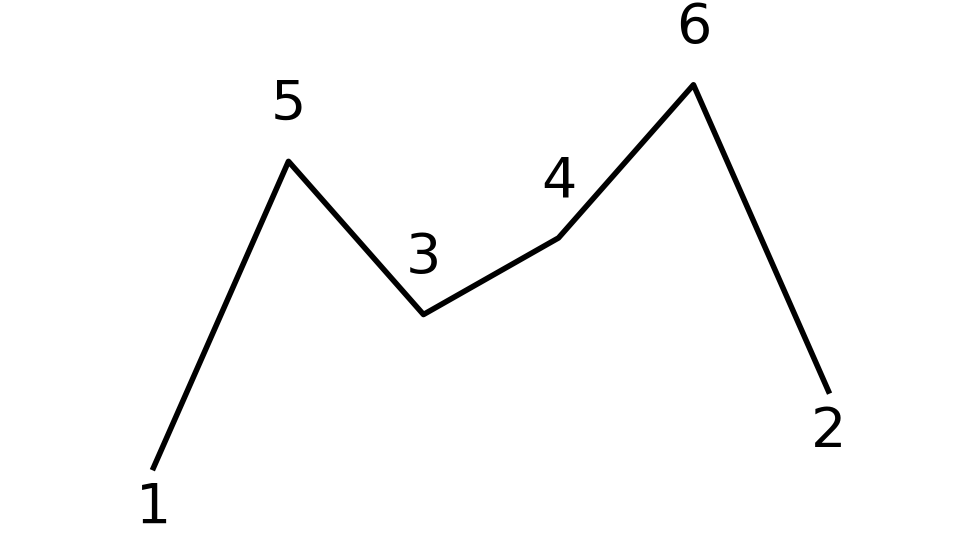
\includegraphics[width=3.5cm]{Introduction/op_P.png} & $T=$ \underline{2 7 4 5 8 3} \underline{1 20 15 16 25 6}  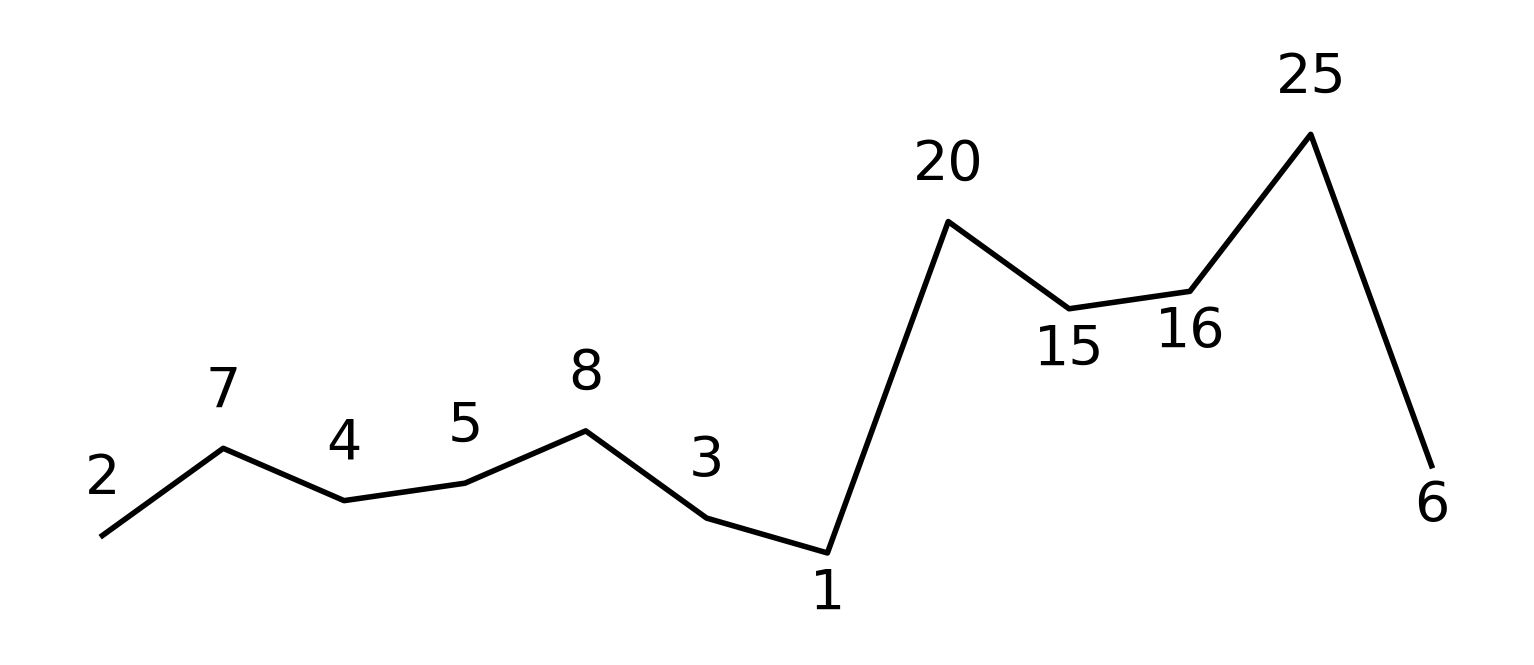
\includegraphics[width=5cm]{Introduction/op_T.png} \\
        %
        Parametrized~\cite{baker1993theory} & $P=$ GATTACAT & $T=$ OPO\underline{POGGODOG}O, {\footnotesize A:O, C:D, G:P, T:G} \\
    \end{tabularx}
    \caption{Example of various model of matching on strings.}
    \label{fig:intro:match_model}
\end{figure}

However, the need for text processing goes far beyond exact matching of patterns. To illustrate this claim, we present models of matching (underlined) relevant to this thesis with their motivations and specify those we study in the following chapter. Figure~\ref{fig:intro:match_model} also provides an example for each matching model.

% Regular expression
One of the oldest and most classic models for more complex queries is \ul{regular expressions} search, introduced by Kleene in 1951~\cite{RM-704}.
% Explain the formalism
The regular expression formalism offers a concise description for sets of strings through recursive combinations of characters from an alphabet $\Sigma$ along with three fundamental operators: concatenation ($\cdot$), union ($|$), and Kleene star ($\ast$).
For two regular expressions $R_1$ and $R_2$ the concatenation $R_1\cdot R_2$ matches any concatenation of a string matching $R_1$ and a string matching $R_2$, the union $(R_1|R_2)$ allows matching any string matching either $R_1$ or $R_2$, and $(R_1)^\ast$ matches any number of repetitions of a string matching $R_1$, including no repetition, i.e. the empty string.
% Application
The use of regular expression gained popularity in the 1970s through their efficient implementation in Unix tools such as awk, grep, or sed.
They have become a crucial tool in many fields such as internet traffic analysis~\cite{4221791,4579527}, databases, data mining~\cite{1000341,10.5555/645927.672035,10.1145/375551.375569}, computer networks~\cite{10.1145/1159913.1159952}, and protein search~\cite{10.1145/369133.369220}.
% automaton
Another way to describe regular expressions is through the Thompson automaton construction~\cite{Thompson_automaton}. This automaton can then be simulated efficiently to test whether a string $T$ is recognized by a regular expression $R$ in $\Oh(|R| \times |T|)$ time.
% Lowerbounds
A series of works~\cite{10.1145/128749.128755,BILLE2008486,10.1007/978-3-642-02927-1_16,10.1007/11786986_56,doi:10.1137/1.9781611973075.104} has focussed on improving the time complexity of regular expression search. However, they only managed to shave off polylogarithmic factors from the $\Oh(|R| \times |T|)$ complexity, and a recent fine-grained complexity approach brought an explanation for this.
Backurs and Indyk~\cite{DBLP:conf/focs/BackursI16} followed by Bringmann, Gr{\o}nlund, and Larsen~\cite{8104068} considered a subclass of regular expressions called ``homogeneous''. A regular expression is ``homogeneous'' if, in the tree representation of the expression, the operators at the same level are equal. For example $R=(P_1|P_2|...|P_d)^\ast$ is homogeneous and searching it corresponds to the Word break problem~\cite{wordbreak1,wordbreak2}. The authors of~\cite{DBLP:conf/focs/BackursI16,8104068} showed that every homogeneous regular expression search either allows for a solution in near-linear time or requires $\Omega((|R| \times |T|)^{1-\alpha})$ time conditioned on the Strong Exponential Time Hypothesis~\cite{IMPAGLIAZZO2001367}. The only exception is the Word break problem which can be solved in $\Oh(n (m \log m)^{1/3}+m)$-time has a matching lower bound up to polylogarithmic factors. Abboud and Bringmann~\cite{DBLP:conf/icalp/AbboudB18} further detailed those lower bounds using an even finer-grained complexity approach.
% Our work
These results give a good understanding of the time complexity of regular expression in the classical setting, however, multiple practical applications need to work with a stream of input. We specify what we mean by a stream later on in this introduction. Therefore, in Chapter~\ref{chap:regexp}, we provide a new space-efficient streaming algorithm for regular expression membership and pattern matching.


% Don't care
Although the versatility of regular expressions makes them widely used in practice across fields, they are notoriously difficult to write for users.
As a simpler alternative, Fischer and Paterson~\cite{fischer1974string} introduced the \underline{``don't care''} pattern matching where a don't care (also called wildcard or gap) symbol, denoted \texttt{?}, can occur in both the pattern and the text, and matches any other character of the alphabet.
% Space seed
This model has been directly applied in the PROSITE~\cite{hulo2006prosite} database of proteins where wildcards are supported. More generally, space seeds~\cite{li2004patternhunter}, a similar concept where only some positions have to be matched, have been used in homology search~\cite{ma2002patternhunter}, alignment~\cite{david2011shrimp2}, assembly~\cite{birol2015spaced}, and metagenomics~\cite{bvrinda2015spaced}.
% Gapped matching
Patterns with don't cares are sometimes~\cite{lewenstein2011indexing} described as $P= P_1g_1P_2g_2 \dots g_\ell P_{\ell+1}$ where $P_1$,$P_2$,\dots,$P_{\ell+1}$ are patterns over the alphabet $\Sigma$ and $g_1,g_2,\dots,g_{\ell}$ are the length of the maximal stretches of \texttt{?}. 
% variable length gap
Naturally this question was later extended to the problem of string matching with \underline{variable length gap}~\cite{bille2012string,bille2014string} where the length of the gaps can vary in intervals $[a_i,b_i]$ for $i\in[1,\ell]$.
% Applications
Note that variable length gaps are also supported by the PROSITE~\cite{hulo2006prosite} database.
% variants
Different variants of the problem have been studied~\cite{kopelowitz2016color,cohen2009range,brodal1999finding}, including a simpler version with just two patterns $P_1$ and $P_2$ and a single gap~\cite{peterlongo2006gapped,iliopoulos2009indexing} and the special case $P_1=P_2$~\cite{muthukrishnan2002efficient,keller2007range}.

% consecutive
In 2016, Navarro and Thankatchan~\cite{NAVARRO2016108} proposed a natural variant to pattern matching with a variable length gap, where given a single pattern $P$ and an interval $[a,b]$, one must report all consecutive occurrences of $P$ starting at positions $(i,j)$ (consecutive meaning no other occurrence in between $i$ and $j$) such that $j-i$ belongs to $[a,b]$. Since, consecutive occurrences have been studied in several publications~\cite{DBLP:conf/fsttcs/BilleGPRS20,cpm/BilleGPS21,DBLP:journals/corr/abs-2304-00887,DBLP:journals/corr/abs-2211-16860}.
% Gapped consecutive matching
Recently Bille et al.~\cite{bille2022gapped} proposed a combination of the gapped and consecutive lines of research: \underline{gapped consecutive matching} where we are given two patterns $P_1$ and $P_2$ as well as an interval $[a,b]$ and must report all consecutive occurrences of $P_1$ and $P_2$ with distance in $[a,b]$.
% Motivations
%This model can be linked to gapped q-grams~\cite{burkhardt2003better} which is an alternative to spaced seeds which were mentioned earlier.
% This thesis
We study gapped consecutive pattern matching in various settings in Chapters~\ref{chap:gapped_index} and~\ref{chap:gapped_pm}, a summary of the contribution is given in Section~\ref{intro:sec:contrib}.
%~\ref{chap:gapped_stream},

Although an in-depth non-standard matching listing is out of scope for this manuscript, for completeness, we detail other models found in the literature, and Table~\ref{fig:intro:match_model} provides exemples for each of the models.
% Degenerate strings
The modelling of flexible and diverse DNA sequences~\cite{comm1970iupac} lead to the model of \underline{degenerate} strings~\cite{abrahamson1987generalized} (also called indeterminate), where each position corresponds to a subset of $\Sigma$.
% (Elastic/Generalised) Degenerate strings
This model has recently been extended in two directions: \underline{elastic degenerate} strings~\cite{iliopoulos2021efficient} where each position is a subset of strings over $\Sigma$ and \underline{generalized degenerate} strings~\cite{alzamel_et_al:LIPIcs:2018:9323} where each position is a subset of strings of $\Sigma^k$, and the length $k$ can vary from position to position.
% Weighted string
Alternatively, when each position is assigned a random variable with values in $\Sigma$ the strings are called \underline{weighted} (or uncertain) and represented by a weight matrix~\cite{thompson1994clustal}, see Table~\ref{fig:intro:match_model} for an example. Then, the cumulative probability that a string occurs at a starting position is the product of the probabilities of the corresponding characters at each position, and a match is often defined by a threshold on that cumulative probability. This model has been used in molecular biology in ``profiles'' that represent multiple aligned strings~\cite{doi:10.1073/pnas.84.13.4355} though they study a slightly different score: $\log \frac{p(x,i)}{p(x)}$ where $p(x,i)$ is the probability that the $i$th character is equal to $x$ and $p(x)$ is the overall frequency of $x$. 
% Abelian/jumbled/many other names 
In the model of \underline{abelian} matching, a string (or a substring) is entirely identified by the characters it contains (with multiplicities), disregarding their order. It stems from the automatic discovery of clusters of genes in genomes where they can occur in a different order but still linked to the same function~\cite{eres2004permutation}, but the same concept has also been used in the context  of using mass spectrometry for DNA assembly~\cite{bocker2003sequencing} where the strings without order are called compomers. This model is also known as jumbled and permutation pattern matching, and several other names, see~\cite{ejaz2010abelian}.
% order preserving
The \underline{order-preserving} model~\cite{kim2014order,kubica2013linear} takes a somewhat opposite approach and says that two strings match if they have the same relative shape: $\forall i,j \in [0,n-1], X[i] < X[j] \leftrightarrow Y[i] < Y[j]$. This matching model aims at capturing the trend detection needed in the stock market and music melody matching problems~\cite{kim2014order}.
%
% Parametrized matching
Another application-driven model is \underline{parametrized strings} or ``p-string'' introduced by Baker~\cite{baker1993theory}, where two strings match if we can transform one into the other by applying a function renaming the parameters, meant to detect code duplication.

\subsection{Periodicity Detection}
\todo[inline]{Work in progress do not review!\\ TODO: Detail}
So far we focussed on matching models where we are given a pattern and text as well as conditions that define a match of the pattern in the text. But another central task in text processing is repetitions detection. By repetitions, we refer to consecutive occurrences of the same fragment. They can be repeated twice (a square), three times (a cube) or more, then represented as a run: a maximal periodic substring. They are needed as a theoretical tool to avoid needless repetitive computations, but they also naturally occur in DNA with an important role in genomic fingerprinting~\cite{Kolpakov2003}.
The study of squares in strings goes back to 1906 with the work of Thue~\cite{thue1906} on the construction of an infinite square free string, in Chapter~\ref{chap:squares} we provide an optimal algorithm for square detection.

% Should also define runs
% Mention palindromes and stuffs ?

\subsection{Similarity Measures}
\todo[inline]{Work in progress do not review!\\ TODO: Complete rewrite and add citations about other model with mismatches}
% Similarity measures
% Explain/illustrate ED, LCS, LCS with $k$ mismatches, DTW
% The notion of robustness of the similarity measure
Although regular expressions are powerful, Bioinformatics\cite{Gusfield1997}, music analysis~\cite{mongeau1990comparison} and plagiarism detection~\cite{lukashenko2007computer} also need relevant and efficient similarity measures such as the Levenshtein distance~\cite{levenshtein1966binary} or Dynamic Time warping distance~\cite{sakoe1978dynamic}. They also often need to report all occurrences with an error bound\cite{landau1986efficient,landau1989fast}: at a distance at most a threshold $\tau$.
We contribute to this line of research in Chapters~\ref{chap:LCS} and~\ref{chap:DTW}.


\subsection{Scalability Issues}\label{sec:intro:scalability}

%%%%%%%%%%%%%%%%%%%%%% Intro scalibility %%%%%%%%%%%%%%%%%%%%%%%%%%%%
 
% But it is not just about the specific model also about scalibility
We discussed so far how string processing tasks have crucial industry-relevant applications, but another major challenge in most applications is the scalability to large datasets.
% Wikipedia
Highly curated datasets generally remain quite small, for example the English pages of Wikipedia (just the text and metadata) take up 20~gigabytes in a compressed format as of 2022~\cite{wikimedia}. In comparison, any form of archival and version history tends to grow much bigger. Just the metadata of revision's history (without the content of the articles) for the Wikipedia English pages takes up 75~gigabytes as of 2022.
% Software Heritage
It is sometimes possible to limit the redundancy in the archival data, for example by using a graph which tracks where the data is repeated multiple times. This is the approach taken by the Software Heritage~\cite{swh-site} project, which aims at keeping an archive of entirety of the software code produced by humanity. The graph structure is especially necessary in this project to reduce code redundancy and reflect the standard use of version history management in software development.
Substantial research and engineering effort~\cite{DBLP:phd/hal/Pietri21} were made to provide an efficient navigation of the graph. 
However, since the code repositories are indexed based on their URLs and metadata, it is not currently feasible to perform a search specifically for occurrences of a particular code snippet\footnote{\setlength\parindent{10pt} A silly but interesting example is~\cite{vii2014if} where the author searched \texttt{"const double epsilon ="} (and equivalents in other languages) on all GitHub repositories to study the value programmers typically chose for epsilon.}.
As of 2023, the graph is limited to 7~terabytes but with the source files the space usage approaches 1~petabyte~\cite{swh-polytechnique}.
% Internet archive
Another example of a large archival project is the internet archive, a non-profit which started saving web pages in 1996 and now holds the history of more than 800 billion web pages through their program: the wayback machine~\cite{web-archive}. This archive takes up more than 70~petabytes, however, one of the limitations is that the search options are limited to the metadata of the websites and not the content of the webpages themselves.


%%%%%%%%%% Bioinformatics
%Intro DNA representation
Large archives also exist in bioinformatics, but the structure of biological sequences is very different from that of code or webpages.
DNA is typically stored as a string over the nucleotide alphabet \texttt{\{A,T,C,G\}} which can be stored using just 2 bits per base. However, this type of storage requires scanning the whole string to search for a pattern. 
At the opposite of the spectrum, a suffix tree enables more efficient sequence analysis but necessitates 10 bytes per base~\cite{navarro2016compact}, which amounting to 30 gigabytes for a human genome containing 3.3 billion bases. 
And thousands of genomes have been sequences through projects such as the 1000 Genomes project~\cite{10002015global} completed in 2015 and the 100K Genomes project~\cite{100Kgenomes} which reached its milestone in 2018. 
A trade-off between those two extremes has been found through the development of compact data structures that exploit redundancy to decrease space usage. For a human genome it allows representing the sequence and its suffix tree using just 4 gigabytes~\cite{navarro2016compact}.
% Redundancy intra genome and intergenome
The redundancy that compact data structures can exploit in genomes can come either from repeated regions in the genome (intra-genome redundancy) or by considering several genomes (from the same specie) that share portions of their genomes (inter-genome redundancy).  
% Reads
However, for DNA, another common data model is the one of reads: when DNA is sequenced, the output is a set of fragments (called \emph{reads}) of the original sequence. Reads can contain sequencing errors, including nucleotide insertions, deletions, and substitutions. The typical length and error rate of the reads vary depending on the sequencing techniques. To be able to reconstruct the original sequence, reads are extracted in such quantities that each position of the original genome is covered multiple times. This means readsets are larger than the assembled genome and even more redundant. In Chapter~\ref{chap:XBWT} we explore this topic for short reads and propose a data structure specifically tailored to the specificities of a sequencing technique. 
% Cheaper = more sequencing
Additionally, the drastic decrease in sequencing cost and increase in throughput since 2008 (faster than expected by Moore's law~\cite{muir2016real}) have lead to higher volumes of DNA being sequenced. 
% ENA
So far, the European Nucleotide Archive has accumulated more than 47 petabytes~\cite{ena} of sequencing data.
% SRA
While the NCBI Sequence Read Archive has more than 73 petabases~\cite{sra} of archive including 38 petabases in open access. However, like for the software heritage project and internet archive, in the ENA and the NCBI, the data is indexed solely based on its metadata.\\
%\todo[inline]{Look for more reasonable size example ? It's unclear if anybody would want to index the entire SRA}

%%%% Astronomical data 
\todo[inline]{Add applications to astronomical data and pulsar detection.}
%\todo[inline]{Add one or several graphs illustrating the growth in data in each field.}

\begin{figure}
    \centering
    \begin{subfigure}[b]{0.45\textwidth}
        \begin{tikzpicture}
            \node (img) {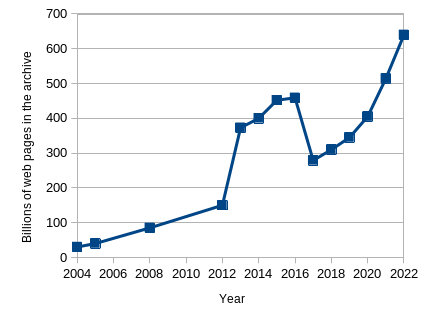
\includegraphics[width=\textwidth]{0_sheets/wayback_machine.png}};
            \node [below right,text width=2.7cm,align=center, fill=white] at (0.25,-0.5){{\fontsize{7pt}{6pt}\selectfont Pages removed due to security concerns.}};
            \draw[->] (1,-0.5) -- (1.3,0.3);
        \end{tikzpicture}
        \caption{The Wayback Machine Archive}
    \end{subfigure}
    \begin{subfigure}[b]{0.49\textwidth}
    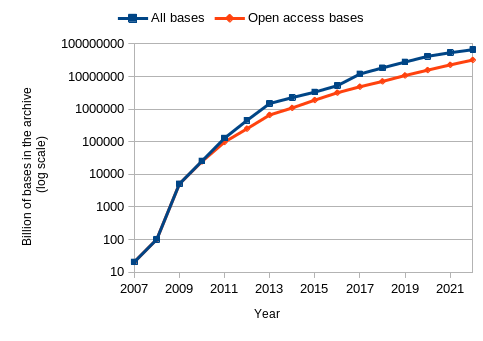
\includegraphics[width=\textwidth]{0_sheets/sra_growth.png}
    \caption{The Sequence Read Archive}
    \end{subfigure}
    \caption{Plots of the database growth for the Wayback Machine~\cite{web-archive-growth} and the Sequence Read Archive~\cite{sra}. The databases are big but also still quickly growing.}
\end{figure}

%%%%%%%%%%%%%%%%%%%%%% Approaches to adress scalibility %%%%%%%%%%%%%%%%%%%%%%%%%%%%
%
It goes without saying that algorithms with quadratic time complexity cannot scale to terabytes and petabytes of inputs. Consequently, the choice of matching model is dictated both by the specific needs of the application and the typical scale of the input.
%
Also note that some applications require \emph{data structures}, which are algorithms where the complexity analysis is split in two parts: the \emph{construction} and the \emph{query}. The construction is generally more expensive and meant to be performed once, whereas the queries are meant to be fast and performed multiple times with varying input-query. For example, Chapters~\ref{chap:gapped_index} and~\ref{chap:XBWT} build data structures.

Several approaches can be used to cope with large amounts of data, such as distributed algorithms that are designed to work on several computers sharing a network (with limited transfer). In this thesis, we focus on a different approach to process massive string data, that of sketching. A \textbf{sketch} is a lossless or lossy compression that keeps only the essential characteristic of the input needed to answer a given query, offering promising scalability potential. Example of sketches include Karp--Rabin fingerprints for lossy compression (see Preliminaries~\ref{sec:prelim:KR}) and Lempel--Ziv factorization for lossless compression (see Preliminaries~\ref{sec:prelim:compress}). 
We will detail in Section~\ref{intro:sec:contrib} how each contribution of this thesis relates to sketching but let us first summarize three general sketch-based approaches (that can sometimes be combined):
%summarize their respective scalability approaches as follows (with some approaches that can be combined): 

\begin{itemize}
\item Compressed input: as mentioned already, highly redundant data can sometimes be represented by a sketch of a more manageable size. 
Consequently, algorithms that can directly operate on the sketch become much more efficient. This is very natural approach as the data is almost always shared in a compressed format, the difficulty focusses on working with the sketch's property and structure. However, it is important to note that not all problems can be solved faster with this approach. For example, Abboud et al.~\cite{abboud2017fine} showed that to compute the longest common subsequence of two strings of uncompressed size $N$, given in a sketch of size $n$, there is a lower bound $(nN)^{1-o(1)}$ assuming the Strong Exponential Time Hypothesis (SETH). 
Very recently, Ganesh et al.~\cite{ganesh2022compression} also showed a lower bound $\Omega(N^{k-1}n)$ conditioned on SETH to compute the median edit distance and length of the longest common subsequence of $k$ strings.
In other words, even if the input is given compressed form, we cannot avoid a high dependency in the uncompressed size. In this thesis, Chapters~\ref{chap:gapped_pm} and~\ref{chap:gapped_index} both take as input a sketch, more precisely a grammar compressed text and their complexities are given as a function of the size of the compressed input.
\item Streaming algorithms: there, the data is considered so large that it can only be handled as a stream. % then it must be processed on the fly without the possibility of going back.
For the pattern matching problem, the pattern and the length of the text are known in advance and can be preprocessed, then the characters arrive one by one and can only be accessed later if they are stored explicitly. 
This model focusses on small space complexity and accounts for every extra space needed apart from the current character. Thus, sketches are crucial to keep the necessary information about the data already seen while limiting space usage.
%This model optimizes both the time per character during the streaming phase and the space complexity which accounts for storing the result of the preprocessing and any space necessary to process the characters.
Chapter~\ref{chap:regexp} is set in this model. %~\ref{chap:gapped_stream}
%
Those streaming algorithms relate in practice to the notion of efficient second-memory algorithms. One of the challenges when dealing with large inputs is the quantity of main memory used, as most computers are still limited to gigabytes of RAM. To circumvent this limitation, programs may resort to working directly from secondary memory as disk space scales at a much cheaper cost than RAM.
It is  common knowledge that random access to disk is very inefficient, however contiguous reads on recent SSD can read gigabytes (between 2.2 and 3.4 Gb) of data per second which is comparable to the speed of most RAM. %which is either comparable to the speed of reading from main memory or only 10 times slower (depending on the model of RAM).
Therefore, an algorithm that uses few random accesses (including streaming algorithms) can be executed directly on disk which allows it to scale to large inputs much more easily. 
%The main issue with this approach is that not all problems admit efficient solutions avoiding random access. For example, given a list and a permutation, returning the permuted list requires to access the elements in the order of the permutation, possibly random. 
We use this approach of streaming on secondary memory to limit main memory usage in Chapter~\ref{chap:XBWT}. The construction of the index is split in phases that read contiguously from disk, process the information (for the next phase or final output) and write to disk.
\item Approximation algorithms: When dealing with very large datasets, it is not always needed to provide precise answers to queries. Allowing for some approximation in the results can enable shortcuts and help bypass lower bounds. There, using sketches in the form lossy compression inherently introduces approximation but allows for even smaller and more efficient representations.
The entire second part of this thesis is dedicated to this approach, and Chapter~\ref{chap:LCS} stands out as a particularly representative example. We treat the problem of the Longest Common Subsequence with approximately $k$ mismatches with a probabilistic algorithm that answer correctly with high probability. %($\geq 1 - \frac{1}{n}$ for an input of size $n$).
\end{itemize}


\chapter*{Preliminaries}
\addcontentsline{toc}{chapter}{Preliminaries}
\chaptermark{Preliminaries}

General string vocabulary


\section{Tries and Suffix trees}

\section{Compression techniques}
What type of compression is used on what problem and why ?
\begin{itemize}
\item RLE
\item Grammar
\item Lempel Ziv
\item BWT
\item State of the art on the equivalence through string attractors
\item Sketches
\end{itemize}


\section{Karp Rabin fingerprint} 
\section{Periodicity and Fine-wilf lemma}
Compact run representation of occ crossing a given position

\section{Streaming pattern matching}
Application to the explanation of Breslauer \& Gallil (needed for both streaming)

\section{Heavy path decomposition}

\part{Complex Queries}\label{part:complex_queries}\mainmatter
%\clearemptydoublepage

\iffalse
% I would like to have this section but for now it is not the priority.
\mainmatter
\chapter{Streaming Gapped Consecutive Matching}\label{chap:gapped_stream}
\subsection{Streaming Pattern Matching}
Application to the explanation of Breslauer \& Gallil, needed for both streaming, though as a black box for regexp.
\fi

\mainmatter
\chapter{Streaming Regular Expression Membership and Pattern Matching}\label{chap:regexp}
%\mainmatter
\newcommand{\rot}{\mathsf{rot}}
\newcommand{\dd}{\mathinner{.\,.\allowbreak}}
\newcommand{\Ohtilda}{\tilde{O}}
\newcommand{\eps}{\varepsilon}
\newcommand{\occ}{\mathsf{occ}}
\newcommand{\Diff}{\mathsf{Diff}}
\newcommand{\Overlap}{\mathsf{Overlap}}
\newcommand{\Zp}{Z_+}

\contextbox{Chapter based on publication}{
This chapter corresponds to the following publication: %\fullcite{}\\
My personal contribution to this work has been the formalization of anchors and proofs of their key properties. I also participated in the overall algorithms design.
TODO: Detail (also in the intro) how it connects to the rest of the thesis and which preliminaries are helpful.
}
\begin{small}
Regular expression search is a key primitive in myriads of applications, from web scrapping to bioinformatics.
A regular expression is a formalism for compactly describing a set of strings, built recursively from single characters
using three operators: concatenation, union, and Kleene star. Two basic algorithmic problems concerning
such expressions are membership and pattern matching.
In the regular expression membership problem, we are given a regular expression $R$ and a string~$T$ of length $n$, and must decide whether $T$ matches~$R$. In the regular expression pattern matching problem, the task to find the substrings of $T$ that match $R$. 

By now we have a good understanding of the complexity of regular expression membership and pattern matching
in the classical setting. However, only some special cases have been considered in the practically relevant streaming
setting:
dictionary matching and wildcard pattern matching. In the dictionary matching problem, we are given a dictionary of $d$ strings of
length at most $m$ and a string $T$, and must find substrings of~$T$ that match one of the dictionary strings. In the wildcard pattern
matching problem, we are given a string $P$ of length $m$ that contains $d$ wildcards, where a wildcard is a special symbol that matches
any character of the alphabet, and a string $T$, and must find all substrings of $T$ that match $P$. Both problems can be solved in the
streaming model by a randomised Monte Carlo algorithm that uses $\Oh(d \log m)$ space [Golan and Porat (ESA 2017), Golan, Kopelowitz
and Porat (Algorithmica 2019)]. 

In the general case, we cannot hope for a streaming algorithm with space complexity smaller than the length of $R$ for either variant
of regular expression search.
The main contribution of this paper is that we identify the number of unions and Kleene stars, denoted by $d$, as the parameter
that allows for an efficient streaming algorithm. This parameter has been previously considered in the classical setting, and
it has been observed that in practice it is significantly smaller than the length of $R$.
We design general randomised Monte Carlo algorithms for both problems that use $\Oh(d^3 \polylog n)$ space
in the streaming setting.

A crucial technical ingredient of our algorithms is an adaptation of the general framework for evaluating a circuit with addition and convolution gates in a space-efficient manner [Lokshtanov and Nederlof (STOC 2010), Bringmann (SODA 2017)], initially designed as a key component of a pseudopolynomial time algorithm for the subset sum problem. We show how to replace the Extended Generalised Riemann Hypothesis in [Bringmann (SODA 2017)] by an application of the Bombieri--Vinogradov theorem to achieve the same bounds (but unconditionally), which might be of independentinterest.
\end{small}

\section{Introduction}
\label{regexp:sec:introduction}
% !TEX root = main.tex

The fundamental notion of regular expressions was introduced back in the 1951 by Kleene~\cite{RM-704}. Regular expression search is one of the key primitives in diverse areas of large scale data analysis: computer networks~\cite{10.1145/1159913.1159952}, databases and data mining~\cite{1000341,10.5555/645927.672035,10.1145/375551.375569}, human-computer interaction~\cite{10.1145/2207676.2208694}, internet traffic analysis~\cite{4221791,4579527}, protein search~\cite{10.1145/369133.369220}, and many others. As such, this primitive is often the main computational bottleneck in these areas and in the pursuit for efficiency has been implemented in many programming languages:
Perl, Python, JavaScript, Ruby, AWK, Tcl and Google RE2, to name just a few.

A regular expression $R$ is a sequence containing characters of a specified alphabet $\Sigma$ and three special symbols (operators): concatenation ($\cdot$), union ($|$), and Kleene star ($\ast$), and it describes a set of strings $L(R)$ on $\Sigma$. For example, a regular expression $R = (a|b)^\ast c$ specifies a set of strings $L(R)$ on the alphabet $\Sigma = \{a,b,c\}$ such that their last character equals $c$, and all other characters are equal to $a$ or $b$. (See formal definition in Section~\ref{sec:prelim}). In this work, we consider two classical formalisations of regular expressions search, regular expression membership and pattern matching. In the regular expression membership problem, we are given a string $T$ of length $n$, and must decide whether $T \in L(R)$ for a given regular expression $R$. In the regular expression pattern matching problem, we must find all positions $1 \le r \le n$ such that for some $1 \le \ell \le r$, the substring $T[\ell \dd r] \in L(R)$. 

Assume that $T$ is read-only, and let $m$ be the length of the regular expression. The classical algorithm by Thompson~\cite{Thompson_automaton} allows to solve both problems in $\Oh(nm)$ time and $\Oh(m)$ space by constructing a non-deterministic finite automaton accepting $L(R)$. Galil~\cite{10.1007/978-3-642-82456-2_1} noted that while the space bound of Thompson's algorithm is optimal in the deterministic setting, the time bound could probably be improved. Since then, the effort has been mainly focused on improving the time complexity of regular expression search. The first breakthrough was achieved by Myers~\cite{10.1145/128749.128755}, who showed that both problems can be solved in $\Oh(mn/\log n + (n+m) \log n)$ time and $\Oh(mn/\log n)$ space. Bille and Farach-Colton~\cite{BILLE2008486} reduced the space complexity down to $\Oh(n^\eps+m)$, for an arbitrary constant $\eps > 0$. This result was further improved by Bille and Thorup~\cite{10.1007/978-3-642-02927-1_16} who showed an algorithm with running time $\Oh(nm(\log\log n)/\log^{3/2} n + n+m)$ time that uses $\Oh(n^\eps+m)$ space. The idea of the algorithms by Myers~\cite{10.1145/128749.128755}, Bille and Farach-Colton~\cite{BILLE2008486}, and Bille and Thorup~\cite{10.1007/978-3-642-02927-1_16} is to decompose Thompson's automaton into small non-deterministic finite automata and tabulate information to speed up simulating the behaviour of the original automaton when reading $T$.
A slightly different approach was taken by 
Bille~\cite{10.1007/11786986_56} who showed that the small non-deterministic finite automata can be simulated directly
using the parallelism built-in in the Word RAM model.
For $w$ being the size of the machine word, Bille showed  $\Oh(m)$-space algorithms with running times~$\Oh(n \frac{m \log w}{w} + m \log w)$ for $m > w$,  $\Oh(n \log m + m \log m)$ for $\sqrt{w} < m \le w$, and~$\Oh(\min\{n+m^2, n \log m+m \log m\})$ for $m \le \sqrt{w}$. Finally, Bille and Thorup~\cite{doi:10.1137/1.9781611973075.104} identified a new parameter affecting the complexity of regular expression search,
which is particularly relevant to this paper.
Namely, they noticed that in practice a regular expression contains $d \ll m$ occurrences of the union symbol and Kleene stars, and showed that regular expression membership and pattern matching can be solved in $\Oh(m)$ space and~$\Oh(n\cdot (\frac{d \log w}{w}+\log d))$ time\footnote{Formally, they consider a parameter $k$ equal to the number of strings in $R$, but it is not hard to see that $k=\Theta(d)$.}.

It is easy to see, however, that in the general case the time complexity of all the algorithms above remains close to ``rectangular'', with some polylogarithmic factors shaved. Recently, fine-grained complexity provided an explanation for this.   
Backurs and Indyk~\cite{DBLP:conf/focs/BackursI16} followed by Bringmann, Gr{\o}nlund, and Larsen~\cite{8104068} considered a subclass of regular expressions which they refer to as ``homogeneous''.  Intuitively, a regular expression is homogeneous, if the operators at the same level of the expression are equal. 
Assume that the alphabet $\Sigma = \{1, 2,\ldots, \sigma\}$. To give a few examples, the following regular expressions are homogeneous: $R_1 = (P_1 | P_2 | \ldots | P_d)$, $R_2 = P_1 (1|2|\ldots|\sigma) P_2 (1|2|\ldots|\sigma) \ldots (1|2|\ldots|\sigma) P_d$, and $R_3 = (P_1 | P_2 | \ldots | P_d)^\ast$, where $P_i$, $1 \le i \le d$, are strings on $\Sigma$, i.e. concatenations of characters in $\Sigma$. \cite{DBLP:conf/focs/BackursI16,8104068} considered both the membership and the pattern matching problems. A careful reader might notice that in the pattern matching setting the expression $R_1$ corresponds to the famous dictionary matching problem~\cite{10.1145/360825.360855} and $R_2$ to pattern matching with wildcards (don't cares) ~\cite{10.5555/889566,10.5555/545381.545468,10.1145/509907.509992,10.5555/795664.796430,CLIFFORD200753}. 
In the membership setting, $R_3$ corresponds to the Word Break problem~\cite{wordbreak1,wordbreak2}. As such, a seemingly simple class of homogeneous regular expressions covers many classical problems in stringology. The authors of~\cite{DBLP:conf/focs/BackursI16,8104068} provided a complete dichotomy of the time complexities for homogeneous regular expressions in both settings. Namely, they showed that in both settings, every regular expression either allows a solution in near-linear time, or requires $\Omega((nm)^{1-\alpha})$ time, conditioned on the Strong Exponential Time Hypothesis~\cite{IMPAGLIAZZO2001367}. The only exception is the Word Break problem in the membership setting, for which~\cite{8104068} showed an $\Oh(n (m \log m)^{1/3}+m)$-time algorithm and a matching combinatorial lower bound (up to polylogarithmic factors).
Later, Abboud and Bringmann~\cite{DBLP:conf/icalp/AbboudB18} took an even more fine-grained approach and
showed that in general, regular expression pattern matching and membership cannot be solved in time $\Oh(nm/ \log^{7+\alpha} n)$ for any constant $\alpha > 0$ under the Formula-SAT Hypothesis. Schepper~\cite{schepper:LIPIcs:2020:12946} extended their result
by revisiting the dichotomy for homogeneous regular expressions,
and showed an $\Oh(nm/2^{\Omega(\sqrt{\log {\min\{n,m\}}}})$ time bound for some regular expressions, and for the remaining ones an improved lower bound of $\Omega(nm/\polylog n)$.  
 
By now we seem to have a rather good understanding of the time complexity of regular expression membership and pattern
matching. However, in multiple practical applications one needs to work with the input arriving as a stream, one character at a time,
without the possibility of going back and retrieving any of the previous characters on demand. This motivates studying
both problems in the streaming model
of computation. In this model, we mostly focus on designing algorithms with small space complexity, and need to account
for storing any information about the input. On the other hand, we allow for randomised algorithms, more specifically
Monte Carlo algorithm returning correct answers with high probability (with respect to the length to the input).
The field of streaming algorithms for string processing is relatively recent but, because of its practical interest, quickly developing.
It started with a seminal paper of  Porat and Porat~\cite{Porat:09}, who showed streaming algorithms for exact pattern matching and for the $k$-mismatches problem. This was followed by a series of works on streaming pattern matching~\cite{DBLP:journals/talg/BreslauerG14,DBLP:conf/esa/CliffordFPSS15,DBLP:conf/esa/GolanP17, DBLP:conf/soda/CliffordFPSS16, starikovskaya:LIPIcs:2017:7320, DBLP:conf/icalp/GolanKP18, gawrychowski_et_al:LIPIcs:2019:10492,clifford2018streaming,DBLP:conf/cpm/GolanKKP20, DBLP:journals/iandc/RadoszewskiS20,DBLP:journals/corr/abs-2106-06037}, search of repetitions in streams~\cite{Ergun:10,stream-periodicity-mismatches, stream-periodicity-wildcards,DBLP:journals/algorithmica/GawrychowskiMSU19, DBLP:conf/cpm/MerkurevS19, DBLP:conf/spire/MerkurevS19, DBLP:conf/cpm/GawrychowskiRS19}, and recognising formal languages in streams~\cite{DBLP:journals/siamcomp/MagniezMN14,ganardi_et_al:LIPIcs:2018:9131, DBLP:conf/lata/GanardiHL18, ganardi_et_al:LIPIcs:2018:8485, ganardi_et_al:LIPIcs:2016:6853, DBLP:conf/mfcs/GanardiJL18, DBLP:journals/tcs/BabuLRV13, franois_et_al:LIPIcs:2016:6355,ganardi_et_al:LIPIcs:2019:11502,bathie_et_al:LIPIcs.ICALP.2021.119}. 

For a general regular expression membership and pattern matching, it is not hard to see that $\Omega(m)$ bits of
space are required by a reduction from Set Intersection.
However, there are at least two interesting special cases of regular expression pattern matching that admit better streaming algorithms.
In the dictionary matching, we are given a dictionary of $d$ strings of length at most $m$ over an alphabet~$\Sigma$ and for each position $r$ in~$T$ must decide whether there is a position $\ell \le r$ such that $T[\ell \dd r]$ matches a dictionary string. A series of work~\cite{Porat:09,DBLP:journals/talg/BreslauerG14,DBLP:conf/esa/CliffordFPSS15,DBLP:conf/esa/GolanP17,DBLP:conf/icalp/GolanKP18} showed that this problem can be solved by a randomised Monte Carlo algorithm in~$\Oh(d \log m)$ space and $\Oh(\log \log |\Sigma|) $ time per character of the text.
In the $(d-1)$-wildcard pattern matching the expression is~$R = P_1 (1|2|\ldots|\sigma) P_2 (1|2|\ldots|\sigma) \ldots (1|2|\ldots|\sigma) P_{d}$, where $P_i$, $1 \le i \le d$ are strings of total length at most $m$ over an alphabet $\Sigma = \{1,2,\ldots,\sigma\}$. Golan, Kopelowitz, and Porat~\cite{DBLP:journals/algorithmica/GolanKP19} showed that this problem can be solved by a randomised Monte Carlo algorithm in $\Oh(d \log m)$ space and $\Oh(d+\log m)$ time per character.
The $d$-wildcard problem is a special case of the $k$-mismatch problem which asks to compute Hamming distances between a pattern and all its alignments to a text for which the Hamming distance does not exceed the given threshold~$k$.
The most space efficient algorithm for the $d$-mismatch problem is by Clifford, Kociumaka and Porat \cite{clifford2018streaming} and implies an algorithm that uses $\Oh(d\log \frac{m}{d})$ words of space and spends $\Oh(\log\frac{m}{d}(\sqrt{d\log d}+\log^3m))$ time per character which is also the most efficient for the $d$-wildcard problem.

In a related work, Ganardi et al.~\cite{ganardi_et_al:LIPIcs:2018:9131,DBLP:conf/lata/GanardiHL18,ganardi_et_al:LIPIcs:2018:8485,ganardi_et_al:LIPIcs:2016:6853} considered a variant of the regular expression membership problem, where the automaton describing the regular expression has constant size, and one must tell, for each position~$r$ of~$T$, whether $T[r-\ell+1\dd r] \in L(R)$, where~$\ell$ is an integer specified in advance (``window'' size). As a culmination of their work, they showed that any randomised Monte Carlo algorithm for this variant of the regular expression membership problem takes either constant, or $\Theta(\log\log \ell)$, or $\Theta(\log \ell)$, or $\Theta(\ell)$ bits of space, and provided descriptions of these complexity classes.

This brings the challenge of identifying a structural parameter of a regular expression that determines whether it admits better
streaming algorithms.
As mentioned earlier, Bille and Thorup~\cite{doi:10.1137/1.9781611973075.104} observed that in practice  
the number $d$ of occurrences of the union symbol and Kleene stars is significantly smaller than the size $m$ of the expression $R$.
Furthermore, both the dictionary matching and the wildcard pattern matching can be casted
as instances of the regular expression pattern matching, and streaming algorithms with space complexity of the form~$\poly(d,\log n)$
are known. The main goal of this paper is to investigate whether this is also the case for the general
regular expression membership and pattern matching.

\subsection{Our results}
We consider the space complexity of regular expression membership and pattern matching in the streaming model of
computation. 
As by now traditional in streaming string processing, we assume that we receive $R$ and $n$ first, preprocess them, and then receive the string $T$ character by character. We do not account neither for the time nor for the space used during the preprocessing stage.
In the membership problem, we must output the answer after having read $T$ entirely, whereas in the pattern matching problem we must decide whether there is a substring $T[\ell \dd r] \in L(R)$ at the moment when we receive the character $T[r]$. 

Our main conceptual contribution is that we identify the small number $d$ of occurrences of the union symbol and Kleene stars
in $R$ as allowing for space-efficient streaming algorithms for regular expression membership and pattern matching.
More specifically, we design randomised Monte Carlo algorithms that solve both problems
using~$\Oh(d^3\polylog n)$ space and $\Oh(nd^5\polylog n)$ time per character of the text (Theorem~\ref{th:memb}).
While it was known that the value of $d$ determines the space complexity in the two special cases of
streaming dictionary matching and wildcard pattern matching, our approach works for any regular expression.
We leave it as an open problem to obtain algorithms with $\poly(d, \log n)$ space complexity and $\poly(d, \log n)$ time complexity. 

On a very high-level, our approach is based on storing carefully chosen subsets of occurrences of the strings appearing in $R$.
As usual in the area, this is easier when the strings are not periodic, that is, any two occurrences of a string $S$ in $T$ must
be more than $|S|/2$ characters apart. Of course, this is not always the case, and the usual remedy is to treat periodic
and aperiodic strings separately (more specifically, in streaming pattern matching algorithms one applies this reasoning
on every prefix of length being a power of 2).
The technical novelty of our algorithms is that we apply this reasoning on $\Oh(\log n)$ levels, thus obtaining
a hierarchical decomposition of a periodic string.
Next, because not all occurrences are stored we need to recover the omitted information.
Very informally, we need to decide whether a substring of $T$ sandwiched between two occurrences of strings $A_1,A_2$ is a label of some run from $A_1$ to $A_2$ in the compact Thompson automaton for $R$, where the period of the substring is equal to the period of
some prefix of length $2^{k}$ of one of the strings. The difficulty is that, while the substring has a simple structure, it could be
very long, and it is not clear how to implement this computation in a space-efficient manner.
We overcome this difficulty by recasting the problem in the language of evaluating a circuit with addition
and convolution gates. This technique was introduced by Lokshtanov and Nederlof~\cite{LokshtanovN10} for designing
a space-efficient solution for the subset sum problem. Later, Bringmann~\cite{Bringmann17} replaced
complex numbers with computation modulo a prime number $p$ to obtain a tighter bound on the time and space complexity.
In more detail, he designed two solutions, one using the Extended Riemann Hypothesis and the other unconditional but
with polynomially higher time and space.
We revisit his approach and show that, in fact, one can replace the Extended Riemann Hypothesis by an application
of the Bombieri--Vinogradov theorem to achieve the same bounds. We believe that this might be of independent interest.
As a consequence of our improvement, we obtain an efficient randomised Monte Carlo algorithm for the following classical problem: given a directed multigraph $G$ with non-negative integer weights on edges, its two nodes $v_1,v_2$, and a number $x$, decide whether there is a walk from $v_1$ to $v_2$ of total weight $x$. Our algorithm requires $x\cdot\poly(|G|,\log x)$ time and $\poly(|G|,\log x)$ space.

The rest of the paper is organised as follows. We first remind the necessary definitions in Section~\ref{sec:prelim}, and in Section~\ref{sec:overview} we give an overview of the main technical ideas we introduced in this paper. We describe the new algorithms for regular expression membership and pattern matching in Section~\ref{sec:algorithms}. Finally, in Section~\ref{sec:paths-in-graph} we describe how to
replace the Extended Riemann Hypothesis with an application of the Bombieri--Vinogradov theorem
in Bringmann's framework and design a space-efficient algorithm for checking if there is a walk of specified weight between
two nodes of a directed multigraph.


\section{Preliminaries}
\label{regexp:sec:prelim}
% !TEX root = main.tex
We assume an integer alphabet $\Sigma = \{1, 2, \ldots, \sigma\}$ with $\sigma$ \emph{characters}. A \emph{string} $Y$ is a sequence of characters numbered from $1$ to $n = |Y|$.  For $1\le i \le n$, we denote the $i$-th character of $Y$ by~$Y[i]$. For $1\le i \le j\le n$, we define $Y[i \dd j]$ to be equal to $Y[i] \dots Y[j]$, called a \emph{fragment} of $Y$. We call a fragment $Y[1] \dots Y[j]$ \emph{a prefix} of $Y$ and use a simplified notation $Y[\dd j]$, and a fragment $Y[i] \dots Y[n]$ \emph{a suffix} of $Y$ denoted by $Y[i \dd]$. We say that a fragment $Y[i \dd j]$ contains a position $k$ if $i \le k \le j$. We denote by $\eps$ the empty string.

We say that $X$ is a \emph{substring} of $Y$ if $X = Y[i \dd j]$ for some $1 \le i \le j \le n$. The fragment $Y[i \dd j]$ is called an \emph{occurrence} of $X$. 
We say that an integer $p$ is a period of $Y$ if for each $1 \le i \le |Y|-p$, $Y[i] = Y[i+p]$. The smallest period of $Y$ is referred to as \emph{the period} of $Y$. We say that $Y$ is \emph{periodic} with period $\rho$ if~$\rho$ is the period of $Y$ and $\rho  \le |Y|/2$. For the period $\rho$ of $Y$, we define the string period of $Y$ to be equal to $Y[1 \dd \rho]$. 

For an integer $k$, we denote the concatenation of $k$ copies of $Y$ by $Y^k$. We say that a string~$X$ is \emph{primitive} if~$X \neq Y^k$ for any string $Y \neq X$ and any integer $k$. Note that the string period of a string is always primitive. 

\begin{definition}[Regular expression]
We define regular expressions over $\Sigma$ as well as the languages they match recursively. Let $L(R)$ be the language matched by a regular expression $R$.
\begin{itemize}
\item Any $a \in \Sigma \cup \{\eps\}$ is a regular expression and $L(a)=\{a\}$.
\end{itemize}
For two regular expressions $A$ and $B$, we can form a new expression using one of the three symbols $\cdot$ (concatenation), $\mid$ (union), or ${}^\ast$ (Kleene star):
\begin{itemize}
\item $A \cdot B$ is a regular expression and $L(A \cdot B)=\{XY, \text{ for } X \in L(A) \text{and } Y \in L(B) \}$;
\item $A \mid B$ is a regular expression and $L(A \mid B)= L(A) \cup L(B)$;
\item $A^\ast$ is a regular expression and  $L(A^*)= \bigcup_{k  \geq 0} \{ X_1 X_2 \dots X_k, \text{ where } X_i \in L(A) \text{ for }$ $1 \leq i \leq k \}$.
\end{itemize}
\end{definition}

\begin{definition}[Thompson automaton~\cite{Thompson_automaton}]
For a regular expression $R$ we define the Thompson automaton of $R$, $T(R)$, recursively. This non-deterministic finite automaton (NFA) accepts all strings $s \in L(R)$.
\begin{itemize}
\item If  $R=a \in \Sigma\cup\{ \eps \} $, $T(R)$ is constructed as in Figure~\ref{fig:Thompson:a};
\item If $R=A \cdot B $, $T(R)$ is constructed as in Figure~\ref{fig:Thompson:AB}. Namely, the initial state of $T(A)$ becomes the initial state of $T(R)$, the final state of $T(A)$ becomes the initial state of $T(B)$, and the final state of $T(B)$ becomes the final state of $T(R)$;
\item If $R=A | B$, $T(R)$ is constructed as in Figure~\ref{fig:Thompson:AorB}. Namely, the initial state of $T(R)$ goes via $\eps$-transitions both to the initial state of $T(A)$ and to the initial state of $T(B)$, and the final states of $T(A)$ and $T(B)$ go via $\eps$-transitions to the final state of $T(R)$;
\item If $R=A^*$, $T(R)$ is constructed as in Figure~\ref{fig:Thompson:A*}. Namely, the initial state of $T(R)$ and the final state of $T(A)$ go via $\eps$-transitions both to the initial state of $T(A)$, and to the final state of $T(R)$. 
\end{itemize}
\end{definition}

\begin{definition}[Compact Thompson automaton]
Given a Thompson automaton $T(R)$, we define the compact Thompson automaton $T_C(R)$ as the automaton obtained from $T(R)$ by replacing every maximal path of transitions labelled by $a_1, a_2, \ldots, a_k \in \Sigma$ by a single transition labelled by $a_1 a_2 \ldots a_k$. The non-empty labels of $T_C(R)$ are called \emph{atomic strings}, and the size of the (multiset) of the atomic strings is defined to be the \emph{size} of $R$.
\end{definition}

Figure~\ref{fig:Thompson_example} gives an example of the Thompson automata for $R = b(ab|b)^*ab$. We note that in general the size of a regular expression is much smaller than the total number of characters in it and is bounded by twice the number of union and Kleene star symbols plus two. The size of a regular expression measures its ``complexity''.

\begin{figure}[!ht]
\begin{subfigure}{0.5\textwidth}
\centering
\begin{tikzpicture}[scale=0.8,every node/.style={scale=0.8}]
    \node[state,initial] (i)   {$i$}; 
   	\node[state,accepting](f)[right=of i] {$f$};
    \path[->] 
    (i) edge [above] node {a} (f);
\end{tikzpicture}
\caption{$T(A)$ for $a\in \Sigma \cup \{ \eps \} $}
\label{fig:Thompson:a}
\end{subfigure}
\begin{subfigure}{0.45\textwidth}
\centering
\begin{tikzpicture}[scale=0.8,every node/.style={scale=0.8}]
    \node[state,initial] (i)   {$i$};
    \node[state](f_1)[right=of i] {};
    \node[state,accepting](f)[right=of f_1] {$f$};
    \draw (1.1,0) ellipse (2cm and 0.8cm);
    \node at (1,-0.5) {$T(A)$};
    \draw (3.5,0) ellipse (2cm and 0.8cm);
    \node at (3.55,-0.5) {$T(B)$};
\end{tikzpicture}
\caption{$T(A\cdot B)$}
\label{fig:Thompson:AB}
\end{subfigure}

\begin{subfigure}[b]{0.5\textwidth}
\centering
\begin{tikzpicture}[scale=0.8,every node/.style={scale=0.8}]
    \node[state,initial] (i)   {$i$};
    \node[state](i_1)[above right=of i] {};
    \node[state](f_1)[right=of i_1] {};
    \node[state](i_2)[below right=of i] {};
    \node[state](f_2)[right=of i_2] {};
    \node[state,accepting](f)[below right=of f_1] {$f$};
    \path[->] 
    (i) edge [above] node {$\eps$} (i_1)
    (i) edge [above] node {$\eps$} (i_2)
    (f_1) edge [above] node {$\eps$} (f)
    (f_2) edge [above] node {$\eps$} (f);
    \draw (3.1,2) ellipse (1.9cm and 0.8cm);
    \node at (3.1,2) {$T(A)$};
    \draw (3.1,-2) ellipse (1.9cm and 0.8cm);
    \node at (3.1,-2) {$T(B)$};
\end{tikzpicture}
\caption{$T(A|B)$}
\label{fig:Thompson:AorB}
\end{subfigure}
\begin{subfigure}[b]{0.45\textwidth}
\centering
\begin{tikzpicture}[scale=0.75,every node/.style={scale=0.7}]
    \node[state,initial] (i)   {$i$};
    \node[state](i_1)[right=of i] {};
    \node[state](f_1)[right=of i_1] {};
    \node[state,accepting](f)[right=of f_1] {$f$};
    \path[->] 
    (i) edge [above] node {$\eps$} (i_1)
    (f_1) edge [above] node {$\eps$} (f);
    \draw [->] (f_1) ..  controls  ($(f_1)+(-0.5,1.5cm)$) and ($(i_1)+(0.5,1.5cm)$) ..  (i_1);
    \node at (2.85,1.4) {$\eps$};
    \draw [->] (i) ..  controls  ($(i)+(0.5,-1.5cm)$) and ($(f)+(-0.5,-1.5cm)$) ..  (f);
    \node at (2.85,-1.1) {$\eps$}; 
    \draw (3.6,0) ellipse (2.2cm and 0.8cm);
    \node at (3.5,0) {$T(A)$};
\end{tikzpicture}
\caption{$T(A^*)$}
\label{fig:Thompson:A*}
\end{subfigure}
\label{fig:thompson}
\caption{Thompson automaton. In each automaton, $i$ and $f$ are the initial and final states, respectively.}
\end{figure}

\begin{figure}[!ht]
\centering
\begin{subfigure}{0.9\textwidth}
\resizebox{\textwidth}{!}{
 \begin{tikzpicture}
    \node[state,initial] (i)   {$i$};
    \node[state] (q1) [right=of i]  {}; 
    \node[state] (i_or)[right=of q1]  {};
    \node[state](i_1)[above right=of i_or] {};
    \node[state] (q2) [right=of i_1]  {};
    \node[state](f_1)[right=of q2] {};
    \node[state](i_2) at (6.25,-1){};
    \node[state](f_2)[right=of i_2] {};
    \node[state](f_or)[below right=of f_1] {};
    \node[state] (q3) [right=of f_or]  {};
    \node[state] (q4) [right=of q3]  {};
   	\node[state,accepting](f)[right=of q4] {$f$};
    \path[->]
    (q1) edge [above] node {$\eps$} (i_or)
    (i_or) edge [above] node {$\eps$} (i_1)
    (i_or) edge [above] node {$\eps$} (i_2)
    (f_1) edge [above] node {$\eps$} (f_or)
    (f_2) edge [above] node {$\eps$} (f_or)
    (f_or) edge [above] node {$\eps$} (q3);
    \path[->]
    (i) edge [above] node {$b$} (q1)
    (i_1) edge [above] node {$a$} (q2)
    (q2) edge [above] node {$b$} (f_1)
    (i_2) edge [above] node {$b$} (f_2)
    (q3) edge [above] node {$a$} (q4)
    (q4) edge [above] node {$b$} (f);
    \draw [->] (f_or) ..  controls  ($(f_1)+(-0.1,2.5cm)$) and ($(i_1)+(0.1,2.5cm)$) ..  (i_or);
    \node at (7.4,3.4) {$\eps$};
   	\draw [->] (q1) ..  controls  ($(q1)+(0.5,-3cm)$) and ($(q3)+(-0.5,-3cm)$) ..  (q3);
    \node at (7.5,-2.1) {$\eps$};
\end{tikzpicture}}
\caption{$T(b(ab|b)^*ab)$}
\end{subfigure}


\begin{subfigure}{0.7\textwidth}
\resizebox{\textwidth}{!}{
 \begin{tikzpicture}
    \node[state,initial] (i)   {$i$};
    \node[state] (q1) [right=of i]  {}; 
    \node[state] (i_or)[right=of q1]  {};
    \node[state](i_1)[above right=of i_or] {};
    \node[state](f_1)[right=of i_1] {};
    \node[state](i_2)[below right=of i_or] {};
    \node[state](f_2)[right=of i_2] {};
    \node[state](f_or)[below right=of f_1] {};
    \node[state] (q3) [right=of f_or]  {};
   	\node[state,accepting](f)[right=of q3] {$f$};
    \path[->]
    (q1) edge [above] node {$\eps$} (i_or)
    (i_or) edge [above] node {$\eps$} (i_1)
    (i_or) edge [above] node {$\eps$} (i_2)
    (f_1) edge [above] node {$\eps$} (f_or)
    (f_2) edge [above] node {$\eps$} (f_or)
    (f_or) edge [above] node {$\eps$} (q3);
    \path[->]
    (i) edge [above] node {$b$} (q1)
    (i_1) edge [above] node {$ab$} (f_1)
    (i_2) edge [above] node {$b$} (f_2)
    (q3) edge [above] node {$ab$} (f);
    \draw [->] (f_or) ..  controls  ($(f_1)+(-0.1,2.5cm)$) and ($(i_1)+(0.1,2.5cm)$) ..  (i_or);
    \node at (6.5,3.4) {$\eps$};
   	\draw [->] (q1) ..  controls  ($(q1)+(0.5,-3cm)$) and ($(q3)+(-0.5,-3cm)$) ..  (q3);
    \node at (6.5,-2.1) {$\eps$};
\end{tikzpicture}}
\caption{$T_C(b(ab|b)^*ab)$}
\end{subfigure}
 \caption{The Thompson automatons of the regular expression $b(ab|b)^*ab$.} 
 \label{fig:Thompson_example}
\end{figure}

\begin{definition}[Occurrence of a regular expression]
We say that a fragment $S[i \dd j]$ of a string~$S$, where $1\le i\le j \le |S|$, is an \emph{occurrence} of a regular expression $R$, if $S[i \dd j] \in L(R)$, or in other words if there is a walk from the initial state of $T_C(R)$ to the final state of $T_C(R)$ such that the concatenation of the labels of the transitions in this walk equals $S[i \dd j]$.
\end{definition}

We will also need a notion of a partial occurrence of $R$. Intuitively, $S[i \dd j]$ is a partial occurrence of $R$ if it is a prefix of a string in $L(R)$, but we will need a more precise definition.

\begin{definition}[Partial occurrence of a regular expression]\label{def:partial_occ_regexp}
We say that a fragment $S[i \dd j]$ of a string $S$, where $1\le i\le j \le |S|$, is a \emph{partial occurrence} of a regular expression $R$ ending with a prefix $P$ of an atomic string $A$, if there is a walk from the initial state of $T_C(R)$ to the endpoint of the transition corresponding to $A$ such that the concatenation of the labels of the transitions in this walk equals $S[i \dd j] A[|P|+1\dd]$. 
\end{definition}


\section{Technical Overview}
\label{regexp:sec:overview}
% !TEX root = main.tex
In this section, we give an overview of the main technical ideas we introduced in this paper. 

\paragraph{Statement of the problems and the model of computation.} Let us start by giving the precise formulation of the regular expression membership and pattern matching problems and reminding the definition of the streaming model of computation. 

\defproblem{\textsc{Regular expression membership and pattern matching}}{ 
Given a string $T$ of length $n$ over an alphabet $\Sigma  = \{1, 2, \ldots, \sigma\}$, where $\sigma = n^{\Oh(1)}$, and a regular expression $R$ over $\Sigma$ of size $d$. In the regular expression membership problem, we must decide whether $T \in L(R)$. In the regular expression pattern matching problem, we must find all positions $1\ \le r \le n$, such that there exists a position $1 \le \ell \le r$ such that $T[\ell \dd r] \in L(R)$.}\\

We work in the streaming model of computation. As it is now standard in the streaming string processing algorithms, we assume to receive $n$ and $R$ first. We do not account neither for the time nor for the space we need to preprocess $R$. After having preprocessed $R$, we receive $T$ as a stream, character by character. At the moment we receive the first character of $T$, the main phase of the algorithm starts. During the main phase, we account for \emph{all} the space and time used. 

\paragraph{Definitions and tools.} 
Let $A_1, A_2, \ldots, A_d$ be the atomic strings of the regular expression $R$. We define $\Pi = \{A_i[1 \dd \min\{2^j, |A_i|\}] : 1\le  i \le d, 0 \le j \le \lceil \log |A_i|\rceil\}$. The prefixes of $A_i$'s that belong to $\Pi$ are called \emph{canonical}.

We can assume that all atomic strings have length at most $n$, otherwise they never appear in the text and we can ignore them. Formally, during the preprocessing phase we delete all transitions $(u,v)$ from $T_C(R)$ that are labelled by atomic strings of lengths larger than $n$. We also assume that $d \le n$, otherwise we can use the following solution:

\begin{claim}\label{claim:few_atomic_strings}
Given a streaming text $T$ of length $n$ and a regular expression of size $d \ge n$. Assume that all atomic strings have length at most $n$ each. There is a deterministic algorithm that solves the membership and the pattern matching problems for $T$ and $R$ in $\Oh(d^2)$ space and $\Oh(d^3)$ time per character of $T$. 
\end{claim}
\begin{proof}
First note that we can afford storing $T$ in full. Second, we build a compact trie on the reverses of the atomic strings of $R$. The trie occupies $\Oh(dn) = \Oh(d^2)$ space. Finally, let $\mathcal{F}$ contain all atomic strings $A$ such that there is an $\eps$-transitions path from the endpoint of the transition labelled by $A$ to the final state of $T_C(R)$.

Define an array $D$ of length $n+1 = \Oh(d)$ such that $D[0]$ contains a singleton set consisting of the starting state of $T_C(R)$ and $D[r]$, $1 \le r \le n$, stores all states $u$ such that $u$ is the end of some transition labelled by an atomic string and $T[1\dd r]$ equals the concatenation of the labels of the transitions in some walk from the starting state of $T_C(R)$ to $u$. Assume that we have constructed $D[1\dd r]$. To compute $D[r+1]$, we use the trie to find the atomic strings $A_1, A_2, \ldots, A_q$ equal to $D[1\dd r+1], D[2\dd r+1], \ldots$  or $D[r+1]$ in $\Oh(r+q)$ time. Note that~$q \le d$. For each atomic string $A_i$, $1 \le i \le q$, labelling a transition $(v,w)$, we add $w$ to $D[r+1]$ if there is a state $u$ in~$D[r+1-|A_i|]$ such that there is an $\eps$-transition path from $u$ to $v$, which can be checked in $\Oh(d)$ time and space. In total, the algorithm spends $\Oh(d^3)$ time to process a character of $T$ ($q = \Oh(d)$, and for each $1 \le i \le q$ the set $D[r+1-|A_i|]$ contains $\Oh(d)$ states). The algorithm reports that $T \in L(R)$ if $D[n]$ contains a state $v$, which is an endpoint of a transition labelled by some $A\in \mathcal{F}$.

In the regular expression pattern matching problem, we define an array $D$ in the following way. As before,~$D[0]$ contains a singleton set consisting of the starting state of $T_C(R)$. For every $1 \le r \le n$, $D[r]$ stores the starting state of $T_C(R)$ and all states $u$ such that $u$ is the end of some transition labelled by an atomic string and $T[\ell \dd r]$, for some $\ell \le r$, equals the concatenation of the labels of the edges in some walk from the starting state of~$T_C(R)$ to $u$. Assume that we have constructed $D[1\dd r]$. To compute $D[r+1]$, we use the trie to find the atomic strings~$A_1, A_2, \ldots, A_q$ equal to $D[1\dd r+1], D[2\dd r+1], \ldots$  or $D[r+1]$ in $\Oh(r+q) = \Oh(d)$ time. For each atomic string $A_i$, $1 \le i \le q$, labelling a transition $(v,w)$, we add $w$ to $D[r+1]$ if there is a state $u$ in $D[r+1-|A_i|]$ such that there is an $\eps$-transition path from $u$ to $v$, which can be checked in $\Oh(d)$ time and space. In total, the algorithm spends $\Oh(d^3)$ time to process a character of $T$. We report all positions $r$ such that $D[r]$ contains a state $v$, which is an endpoint of a transition labelled by some $A\in \mathcal{F}$.
\end{proof}

From now on, we assume that all atomic strings have length at most~$n$, and that $d \le n$. 
For a string $P$ and a text $T$, denote by $\occ(P,T)$ the set of the ending positions of the occurrences of $P$ in $T$. Our solutions for streaming regular expression membership and pattern matching are very similar, the main difference is how we define a witness:

\begin{definition}[Witness (Membership)]\label{def:witness-memb}
Let $P$ be a canonical prefix of an atomic string, and $r \in \occ(P,T)$. 
We say that $r$ is a \emph{witness} if $T[1 \dd r]$ is a partial occurrence of $R$ ending with $P$.  
\end{definition}

\begin{definition}[Witness (Pattern matching)]\label{def:witness-matching}
Let $P$ be a canonical prefix of an atomic string, and $r \in \occ(P,T)$. 
We say that $r$ is a \emph{witness} if there exists a position $1 \le \ell \le r$ such that $T[\ell \dd r]$ is a partial occurrence of $R$ ending with $P$.  
\end{definition}

\noindent
We exploit the following algorithm, which we refer to as the pattern matching algorithm\footnote{One could also use one of the streaming dictionary matching algorithms (see the introduction), but this does not change the final complexity and makes the description of the algorithm more complex.}:

\begin{thm}[{cf.~\cite[Theorem 2]{Porat:09}}]\label{th:pattern_matching}
Given a pattern of length at most $n$ and a text $T$ of length $n$ over an alphabet of size $n^{\Oh(1)}$. There exists a randomised Monte Carlo streaming algorithm that uses $\Oh(\log n)$ space and~$\Oh(\log n)$ time per character of the text. When it receives $T[i]$, it says whether $i \in \occ(P,T)$. The algorithm is correct with high probability.\footnote{With high probability means with probability at least $1-1/n^c$ for any predefined constant $c>1$.}
\end{thm}
\noindent
We also make use of the following well-known fact:
\begin{fact}[Fine and Wilf's periodicity lemma~\cite{Fine1965}]\label{fact:fine_wilf}
If a string $X$ has two periods of length~$p$ and~$q$ and $p+q \le |X|$, then $X$ also has a period of length $\gcd(p,q)$.
\end{fact}

\paragraph{Intuition: non-periodic case.} 
To give intuition behind our solutions, consider a very simple case when every canonical prefix is not periodic. We start with the following simple observation:

\begin{observation}\label{obs:few_occ}
By Fact~\ref{fact:fine_wilf}, if $P$ is not periodic, there can be at most two occurrences of $P$ in a string of length $\le 2|P|$.
\end{observation}

Therefore, if none of the strings in $\Pi$ is periodic, we can use the following approach. For each $P \in \Pi$ and $T$, we run the pattern matching algorithm and at any moment store the two most recent witnesses for $P$ discovered by the algorithm (for membership, witness are defined as in Definition~\ref{def:witness-memb}, and for pattern matching as in Definition~\ref{def:witness-matching}). When the algorithm discovers a new position $r \in \occ(P,T)$, we must decide whether it is a witness. Let $P = A[1 \dd \min\{2^k, |A|\}]$, where $A$ is an atomic string. 

If $k = 0$, we consider the starting node $u$ of the transition in the compact Thompson automaton $T_C(R)$ labelled by $A$. Suppose that there is an $\eps$-transitions path from the endpoints of the transitions labelled by atomic strings $A_{i_1}, A_{i_2}, \ldots, A_{i_j}$ to $u$. We then check if $(r-1)$ is a witness for at least one of $A_{i_1}, A_{i_2}, \ldots, A_{i_j}$. If it is, then $r$ is a witness. Importantly, if $r-1$ is a witness for $A_{i_{j'}}$, $1 \le j' \le j$, it is the most recent one and is stored in the memory of the instance of the pattern matching algorithm for $A_{i_{j'}}$ and $T$. Suppose now that $k \ge 1$. We then must check whether $(r-2^{k-1})$ is a witness for $A[1\dd 2^{k-1}]$. If it is, then $r$ is a witness for $P$. Note that by Observation~\ref{obs:few_occ}, if $(r-2^{k-1})$ is a witness for $A[1\dd 2^{k-1}]$, it is one of the two most recent ones and will be stored by the pattern matching algorithm for $A[1\dd 2^{k-1}]$.

Let $\mathcal{F}$ contain all atomic strings $A$ such that there is an $\eps$-transitions path from the endpoint of the transition labelled by $A$ to the final state of $T_C(R)$. In the regular expression pattern matching problem, we report all positions $r$ such that $r$ is a witness in $\occ(A,T)$ for some $A\in \mathcal{F}$. In the regular expression membership problem,~$T \in L(R)$ if $n$ is a witness for $\occ(A,T)$, for some $A\in \mathcal{F}$.

We do not provide the formal analysis of the algorithm, as we only give it for intuition, but it is easy to see that it uses $\Oh(d^2 \log^2 n)$ space and $\Oh(d \log^2 n)$ time per character of the text (recall that we do not account for the time spent during the preprocessing phase). As all atomic strings have length at most $n$ and $d \le n$, the algorithm is correct with high probability by Theorem~\ref{th:pattern_matching}.

\paragraph{General case: main technical contributions.}
In general, unfortunately, some of the canonical prefixes are periodic we can no longer use Observation~\ref{obs:few_occ}. However, the following generalisation holds:

\begin{observation}\label{obs:few_progressions}
By Fact~\ref{fact:fine_wilf}, if for a string $P$ and a string $X$, $X \le 2|P|$, we have $|\occ(P,X)| > 2$, then $P$ is periodic and the set $\occ(P,X)$ can be represented as an arithmetic progression with difference $\rho$, where $\rho$ is the period of $P$. \footnote{Note that when $|\occ(P,X)| \le 2$, we can represent $\occ(P,X)$ as at most two (degenerate) arithmetic progressions of length~$1$, we will use this fact to simplify the description of the algorithms.}
\end{observation}

Observation~\ref{obs:few_progressions} gives the idea behind our approach for the general case. By this observation, we obtain that every $r \in \occ(P,T)$, where $P$ is a canonical prefix of some atomic string periodic with period $\rho$, belongs to a fragment of form $(\Delta(P))^k$, where $\Delta(P) = P[|P|-\rho+1 \dd]$ and $k$ is an integer. 
Instead of storing the last two witnesses for each canonical prefix, we would like to store the witnesses in the last two fragments of form $(\Delta(P))^k$. However, the number of such witnesses can be large. Our main technical novelty is a compressed representation of such witnesses. We give a high-level overview of the approach we use for the membership problem, our solution to the regular expression pattern matching problem is similar. We show that for each fragment of form $(\Delta(P))^k$ it suffices to store a small, carefully selected subset of witnesses that belong to this fragment. The remaining ones can be restored in small space at request. 

Consider a witness $r \in \occ(P, T)$, where $P \in \Pi$. By definition, there is a partition $T[1\dd r] = T[\ell_1\dd r_1] T[\ell_2 \dd r_2]$ $\ldots T[\ell_m \dd r_m]$ such that each fragment in the partition, except for the last one, is an atomic string, and the last one equals $P$. Furthermore, by Observation~\ref{obs:few_progressions}, $r$ must belong to some fragment $F = T[i \dd i + k \rho -1] = (\Delta(P))^k$. Let $m'$ be the index of the first fragment such that $r_{m'} \ge i$. Consider the fragment $W = T[\ell_{m''} \dd r_{m''}]$, $m' \le m'' \le m$, containing a position $i+2\rho-1$ (we call this position an ``anchor''). Note that $W$  is a canonical prefix of some atomic string and $r_{m''} \in \occ(W, T)$ is a witness. If there are a few witnesses $t \in \occ(W, T)$ such that $T[t-|W|+1,t]$ contains the anchor $i+2\rho-1$, we can store them explicitly. Otherwise, there is a periodic fragment containing $i+2\rho-1$, and we can recurse for it by choosing a new anchor close to its starting point. We choose the definition of anchors (see Section~\ref{regexp:sec:anchors}) so that the recursion stops in a logarithmic number of steps and for some of the anchors there is a witness that we store explicitly for this anchor. 

To summarize, the idea of the compact representation of witnesses that belong to a fragment of form $(\Delta(P))^k$ is to choose a logarithmic set of anchors close to the starting point of the fragment, and for each of these anchors to store a constant number of witnesses for each canonical prefix in~$\Pi$.  Suppose now that $r \in \occ(P,T)$, where~$P$ is a canonical prefix of an atomic string $A$, $r$ belongs to a fragment $F = T[i \dd i + k \rho -1] = (\Delta(P))^k$. To decide whether it is a witness we use the following approach. From above we know that $r$ is a witness iff there is a witness $r' \in \occ(A',T)$, where $A'$ is an atomic string, that we store in the compact representation of witness in $F$, and there is a path in $T_C(R)$ from the ending node of the transition labelled by $A'$ and to the starting node of the transition labelled by $A$ such that the concatenation of the strings on the edges of the path equals $T[r'+1\dd r-|A|]$ (which is a substring of $(\Delta(P))^k$). Unfortunately, it is not clear how to verify this condition in a straightforward way as we do not have random access neither to $\Delta(P)$, nor to the strings on the edges of $T_C(R)$. Instead, using anchors again, we show that verifying this condition can be reduced to the following question, where $G$ is a graph of size $\poly(d, \log n)$ (see Lemma~\ref{lm:restore_witnesses} for details):

\defproblem{\textsc{Walks in a weighted graph}}{ 
Given a directed multigraph $G$ with non-negative integer weights on edges, two nodes and a number $x$, decide if there is a walk from the first node to the second one of total weight $x$.}\\

\paragraph{Walks in a weighted graph and circuits.} In Section~\ref{regexp:sec:paths-in-graph}, we show the following theorem:

\begin{thm}\label{thm:detecting_walk_specific_weight}
 There exists an algorithm which, given a directed multigraph $G$ with non-negative integer weights on edges, its two nodes $v_1$ and $v_2$ and a number $x$,  decides if there is a walk from $v_1$ to $v_2$ of total weight $x$ in~$\Oh((|E(G)|+|V(G)|^3)x\polylog x)$ time and $\Oh((|E(G)|+|V(G)|^3)\polylog x)$ space and succeeds with probability at least $1/2$.
\end{thm}

Let $N=|V(G)|$.
For the simpler case when the graph is unweighted, we could use a folklore approach and compute the $x$-th power of the adjacency matrix in $\Oh(N^3\log x)$ time and $\Oh(N^2)$ space.
In order to handle arbitrary weights of edges, we compute the arrays $C_k$ of bit-vectors of length $x+1$, where $C_k[u,v][d]$ stores a bit indicator of whether there exists a walk from $u$ to $v$ in $G$ of at most $2^k$ edges of total weight exactly $d$. The following formula holds:
$$C_k[u,v][d]=\bigvee_{\substack{w\in V(G) \\  i\in \{0,\ldots,d\}}} C_{k-1}[u,w][i] \wedge C_{k-1}[w,v][d-i]$$
Using the fast Fourier transform to compute the convolutions, we obtain an algorithm with $\Oh(N^3x\log^2x)$ time and space $\Oh(N^2x)$. 

In our application, $x$ can be equal to $n$, and the approach above uses $\Omega(n)$ space, which is prohibitive. 
In order to improve the space complexity, we represent the above computations as a circuit with binary \textsc{Or} and \textsc{Convolution}$_x$ gates operating on bit-vectors of length $x+1$.
Every element $C_k[u,v]$ requires a separate gate and while computing its value we need to perform $N$ convolutions, for every possible intermediate node $w$, so in total there are $\Oh(N^3\log x)$ gates.
The \textsc{Convolution}$_x$ gates store only the first $x+1$ bits of the results, as we never need paths of total weight larger than $x$.
We are interested only in a single bit of output of the circuit, namely $C_{\lceil\log x\rceil}[v_1,v_2][x]$. If there were only \textsc{Or} gates in the circuit, we could store only the $x$-th element at each gate.
In order to handle also \textsc{Convolution}$_x$ gates, we use the discrete Fourier transform over a suitably chosen ring.

We use the technique introduced by Lokshtanov and Nederlof \cite{LokshtanovN10} and then modified
Bringmann \cite{Bringmann17} to work with numbers modulo $p$ instead of complex numbers.
Informally, they show that if we operate on $\mathbb{Z}_p^t$ (vectors of length $t$ with elements in $\mathbb{Z}_p$ for suitably chosen $p$ and $t$) instead of the bit-vectors, we can compute $out(C)[x]$, the $x$-th element of the output of the circuit $C$ in $\Oh(|C|t\polylog p)$ time and $\Oh(|C|\log p)$ space (see details in Theorem~\ref{thm:circuits_framework}).
However, there are technical difficulties that we need to overcome to apply their technique to our solution. The approach of Bringmann \cite{Bringmann17} requires that $t>x$ and $\mathbb{Z}_p$ contains a $t$-th root of the unity.
The main difficulty is to choose these numbers as small as possible as they directly affect the complexity of the algorithm.
This question was also faced by Bringmann~\cite{Bringmann17}, who showed two variants of the framework, one using the Extended Riemann Hypothesis and the other unconditional but with polynomially higher time and space, which is not good enough for our streaming application. By using Bombieri--Vinogradov theorem (see details in Theorem~\ref{thm:bombieri}) and facts about counting primes in arithmetic progressions, we obtain an unconditional time bound comparable to that of Bringmann that assumes the Extended Riemann Hypothesis.

%Secondly\todob{Aren't the two difficulties too easy to mention?}, in order to use the properties of discrete Fourier transform, we need to guarantee that convolutions do not overflow. In other words, we need to ensure that we never obtain a path of total weight exceeding $t$. We achieve that by including longer edges only in the later matrices $C_k$. More precisely, at the $k$-th step we consider all walks of weight bounded by $(1+\eps)^k$, some walks of weight bounded by $(1+\eps)^{k(1+2\log(1+\eps)}$ and no walks of larger weight, where $\eps = \frac{1}{\log x}$. Finally, we operate modulo $p$, which may result in false positive errors if the answer is congruent to 0 modulo $p$. We show that if we didn't apply modulo $p$ at every step, all the values would be bounded by $2^{\Oh(x\log x)}$. This suffices to obtain the desired bounds.

\section{Regular Expression Membership and Pattern Matching}\label{sec:regexp}
In this section, we address the problems of regular expression membership and pattern matching in the streaming model of computation. In Section~\ref{regexp:sec:anchors}, we introduce a notion of \emph{anchors} that is the key to achieving the desired space complexity. In Section~\ref{regexp:sec:algorithms}, we describe the algorithms.

\subsection{Anchors}
\label{regexp:sec:anchors}
% !TEX root = main.tex
In this section we define the notion of anchors that will allow us to store all occurrences (partial or not) of regular expressions detected by the algorithm efficiently. 

%\begin{corollary}[Of Fact~\ref{fact:fine_wilf}]\label{cor:}
%For a primitive string $X$ of length $x$, a string $D = XX$ can contain only two occurrences of string $X$, $D[1\dd x]$ and $D[x+1\dd 2x]$.
%\end{corollary}

\begin{definition}[Anchors]\label{def:anchors}
Consider a periodic string $W$ with period $\rho$. Set the anchor $a_0 = 2\rho$ and the period~$\rho_0 = \rho$. Suppose that $(a_r, \rho_r)_{r = 0}^{q-1}$ are defined. We define $(a_{q}, \rho_{q})$ recursively. Consider the set $S$ of fragments $W[i \dd j]$ of $W$ satisfying the following properties:
\begin{enumerate}
\item $W[i \dd j]$ contains $a_{q-1}$ and is periodic with period $\pi < \rho_{q-1}$;
\item $i+4\pi-1 \le a_{q-1}$ (there are at least four repetitions of the string period of $W[i \dd j]$ before $a_{q-1}$);
\item $a_{q-1} \le j-4\pi-r$, where $r = (j-i+1) \pmod \pi$ (there are at least four repetitions of the string period of $W[i \dd j]$ after $a_{q-1}$).
\end{enumerate}
Let $i_q = \min\{i : W[i\dd j] \in S\}$ and $j_q = \max\{j : W[i_q\dd j] \in S\}$. If $W[i_{q} \dd j_{q}]$ is undefined, recursion stops. Otherwise, $\rho_q$ is defined to be the period of $W[i_q \dd j_q]$ and $a_{q} := i_{q}+2\rho_{q}-1$. 

Let $\A(W) = \{a_0, a_1, \ldots, a_{Q}\}$, where $(a_Q,\rho_Q)$ is the last defined anchor-period pair. We call $\A$ the \emph{generator set of anchors} of $W$. Define $\A^\ast(W) = \left[\bigcup_{\Delta \in \mathbb{Z}_+} (\A(W) + \Delta \cdot \rho)\right] \cap [1, |W|-2\rho]$. We refer to $\A^\ast$ simply as the \emph{set of anchors} of $W$. For an illustration, see Fig.~\ref{fig:anchors}.
\end{definition}

\begin{figure}[ht!]
\ctikzfig{Part_One/streaming_regex_pattern_matching/figures/fig1}
\caption{Anchors of a periodic string $W$ with period $\rho$.}
\label{fig:anchors}
\end{figure}

(In the next section we slightly abuse notation and extend the notion of the set of anchors to infinite strings in a natural way, i.e. for an infinite string $W$ with period $\rho$ the set $\A^\ast(W) = \left[\bigcup_{\Delta \in \mathbb{Z}_+} (\A(W) + \Delta \cdot \rho)\right]$.) 
We first show that the generator set of anchors has logarithmic size:

\begin{lemma}\label{lm:anchors}
Let $W$ be a periodic string with period $\rho$. We have $|\A(W)| = \Oh(\log \rho)$. 
\end{lemma}
\begin{proof}
Let $\A(W) = \{a_0, a_1, \ldots, a_Q\}$. For each $0 \le q \le Q$, let $W[i_q \dd j_q]$ be the fragment associated with $a_q$, and~$\rho_q$ be its period. (In particular, for $q = 0$ we have $i_0 = 1$, $j_0 = |W|$, $\rho_0 = \rho$.) We show that for each $1 \le q \le Q$ we have $|W[i_q \dd j_q]| \le 2 \rho_{q-1}$. This implies, in particular, that $|W[i_q\dd a_{q-1}]| \le  2 \rho_{q-1}$ and therefore $\rho_q \leq \rho_{q-1} / 2$. The lemma follows immediately. 

Fix $0 \le q \le Q$. Assume by contradiction that $|W[i_q \dd j_q]| > 2 \rho_{q-1}$. We then have that $W[i_q \dd j_q]$ has periods $\rho_{q-1}$ and $\rho_q$ and $\rho_{q-1}+\rho_q < |W[i_q \dd j_q]|$. Hence, $W[i_q \dd j_q]$ is periodic with period $\pi = \gcd(\rho_{q-1},\rho_q)$ by Fact~\ref{fact:fine_wilf}. The substring $W[i_q \dd j_q]$ contains a full copy of $W[i_{q-1} \dd i_{q-1}+\rho_{q-1}-1]$. Therefore, $W[i_{q-1} \dd i_{q-1}+\rho_{q-1}-1]$ has a period $\pi$, which implies that it equals $(W[i_{q-1} \dd i_{q-1}+\pi-1])^{\rho_{q-1}/\pi}$, i.e. the string period of $W[i_{q-1} \dd j_{q-1}]$ is not primitive, a contradiction. 
\end{proof}


\begin{definition}
Let $W$ be a periodic string with period $\rho$. We say that a fragment $F = W[i \dd j]$ is anchored by an anchor $a \in \A^\ast(W)$ if $i \leq a \leq j$ and for any strings $U \in \Sigma^\ast, V \in \Sigma^\rho$ such that $V \neq W[1 \dd \rho]$ there are at most eight occurrences of $F$ in $UV(W[1\dd j])$ containing the anchor (i.e., containing $|U|+|V|+a$). 
\end{definition}

\begin{lemma}\label{lm:anchors_catch_partial_match}
Let $W$ be a periodic string with period $\rho$. Consider a fragment $W[\ell \dd r]$ of length at least $4 \rho$ and a partitioning $W[\ell \dd r] = W[\ell_1 \dd r_1] W[\ell_2 \dd r_2] \ldots W[\ell_k \dd r_k]$. 
\begin{enumerate}[label=\textrm{(\alph*)}]
\item There exists $1 \le k' \le k$ such that $W[\ell_{k'} \dd r_{k'}]$ is anchored by an anchor $a \in \A^\ast(W) \cap [r-4\rho+1, r]$.\label{it:anchor_gen}
\item If, in addition, $1 \le \ell \le 2 \rho$, there exists $1 \le k' \le k$ such that $W[\ell_{k'} \dd r_{k'}]$ is anchored by an anchor $a \in \A^\ast(W) \cap [1, 4\rho]$.\label{it:anchor_beg}
\end{enumerate}
\end{lemma}
\begin{proof}
The high-level idea of the proof of~\ref{it:anchor_gen} and~\ref{it:anchor_beg} is as follows. Let $\A(W)= \{a_0,a_1, \ldots a_Q \}$. For every~$0 \le q \le Q$ and an integer $\Delta > 0$ to be determined later, define $a_q^\Delta := a_q +\Delta \cdot \rho$. Let $F_q=W[\ell_{k_q},r_{k_q}]$ be the fragment that contains $a_q^{\Delta}$. We show that either $F_q$ is anchored by $a_q^{\Delta}$ or $q < Q$, which yields the lemma. We exploit two auxiliary claims:

\begin{claim}\label{claim:many_reps}
Let $\pi$ be the period of $F_q$, $0 \le q \le Q$. If $F_q$ is not anchored by $a_q^\Delta$, then there exist $U \in \Sigma^\ast, V \in \Sigma^\rho$ with $V \neq W[1 \dd \rho]$ such that there is a fragment $S[p \dd t]$ of the string $S = UV(W[\dd r_q])$ satisfying the following properties:
\begin{enumerate}
\item $p \le |U|+|V|+a_q^\Delta \le t$ (the fragment contains the anchor);
\item $S[p \dd t]$ is periodic with period $\pi$;
\item $p+7\cdot \pi \le |U|+|V|+a_q^\Delta$ (there are at least seven repetitions of the string period of the fragment before the anchor);
\item $|U|+|V|+a_q^\Delta \le t-6\pi-r$, where $r = t-p+1 \pmod \pi$ (there are at least six repetitions of the string period of the fragment after the anchor). 
\end{enumerate}
\end{claim}
\begin{proof}
Let $U \in \Sigma^\ast, V \in \Sigma^\rho$ with $V \neq W[1 \dd \rho]$ such that there are least eight occurrences of $F_q$ in $S = UV(W[1 \dd r_q])$ containing $a := |U|+|V|+a_q^\Delta$. Let the last eight occurrences be $S[p_k \dd t_k]$, $1 \le k \le 8$. As all occurrences contain $a$, the length of $S[p_1 \dd t_8]$ is at most $2|F_q|$. By Observation~\ref{obs:few_progressions}, we obtain that $S[p_1 \dd t_8]$ is periodic with period $\pi$, $p_k = p_1 + (k-1) \pi$, and $t_k = t_1 + (k-1) \pi$. As $p_8 = p_1+7\pi \le a$,  we have $S[p_1 \dd a] \ge 7 \pi$. On the other hand, $t_2-r+1 \ge t_1+1 \ge a+1$. Therefore, $|S[a+1 \dd t_8-r]| \ge |S[t_2-r+1 \dd t_8-r]| \ge 6\pi$. By taking $p = p_1$ and $t = t_8$, we obtain the claim. For an illustration, see Fig.~\ref{fig:claim_many_reps}.
\end{proof}

\begin{figure}[ht!]
\centering
\ctikzfig{Part_One/streaming_regex_pattern_matching/figures/claim1}
\caption{Illustration of Claim~\ref{claim:many_reps}.}
\label{fig:claim_many_reps}
\end{figure}

\begin{claim}\label{claim:next_level}
Assume that $q \ge 0$ and that the period of $F_q$ is $\pi < \rho_q$. If $F_q$ is not anchored by $a_q^\Delta$, then $q < Q$. 
\end{claim}
\begin{proof}
By Claim~\ref{claim:many_reps}, there exist $U \in \Sigma^\ast, V \in \Sigma^\rho$ with $V \neq W[1 \dd \rho]$ such that there is a fragment $S[p \dd t]$ of the string $S = UV(W[\dd r_q])$ periodic with period $\pi$ that contains $a: = |U|+|V|+a_q^\Delta$ and such that there are at least six repetitions of the string period before and after $a$.

Let us show that $a-2\rho_q+1 \le p < t \le a+2\rho_q$. Suppose by contradiction that $p < a-2\rho_q+1$. We have that $S[a-2\rho_q+1 \dd a] = W[a_q^\Delta-2\rho_q+1 \dd a_q^\Delta]$ (note that by definition $a_q^\Delta \ge 2 \rho_q$ for any~$\Delta$). Furthermore,~$W[a_q^\Delta-2\rho_q+1 \dd a_q^\Delta]$ has periods $\rho_q$ (by definition of $i_q$ and $a_q^\Delta$) and~$\pi$ (by the assumption). By Fact~\ref{fact:fine_wilf}, $W[a_q^\Delta-2\rho_q+1 \dd a_q^\Delta]$ has a period $\gcd(\rho_q, \pi) < \rho_q$. As $W[a_q^\Delta-2\rho_q+1 \dd a_q^\Delta]$ contains a full copy of the string period of $W[i_q \dd j_q]$, we obtain that it is not primitive, a contradiction. (See Fig.~\ref{fig:claim_next_level}). To show that~$t \le a+2\rho_q$, note that $S[a+1 \dd a+2\rho_q] = W[a_q^\Delta+1 \dd a_q^\Delta+2\rho_q]$, $a_0^\Delta+2\rho \le |W|$ and, for $q\ge 1$, $a_q^\Delta+2\rho_q \le a_{q-1}^\Delta$ by definition of $i_q$ and $a_q$. Therefore, for all $q \ge 0$, $W[a_q^\Delta+1 \dd a_q^\Delta+2\rho_q]$ is periodic with period~$\rho_q$. The rest of the argument is analogous. 

From $a-2\rho_q+1 \le p < t \le a+2\rho_q$ and the fact that $S[p \dd t]$ contains at least six repetitions of its string period before and after $a$, we obtain that $i_{q+1}, j_{q+1}$ and hence $a_{q+1}, \rho_{q+1}$ are well-defined, which completes the proof of the claim.  
\end{proof}

\begin{figure}
\centering
\ctikzfig{Part_One/streaming_regex_pattern_matching/figures/claim2}
\caption{Illustration of the proof of Claim~\ref{claim:next_level}, case $p < a-2\rho_q+1$.}
\label{fig:claim_next_level}
\end{figure}
\noindent
We are now ready to show~\ref{it:anchor_gen} and~\ref{it:anchor_beg}. 

\begin{enumerate}[label=\textrm{(\alph*)}]
\item Let $\Delta \le \lfloor |W|/\rho\rfloor-2$ be the smallest integer such that $a_0+\Delta \cdot \rho \ge r-4\rho$. Note that $\Delta$ is well-defined. 
 Consider an anchor $a_0^\Delta = a_0+\Delta \cdot \rho \in \A^\ast(W) \cap [r-4\rho+1, r]$. Let $F_0 = W[\ell_{k_0} \dd r_{k_0}]$ be the fragment that contains $a_0^\Delta$ and~$\pi$ be its period. If $F_0$ is anchored by $a_0^\Delta$, we are done. Otherwise, by Claim~\ref{claim:many_reps}, there exist~$U \in \Sigma^\ast, V \in \Sigma^\rho$ with $V \neq W[1 \dd \rho]$ such that there is a fragment $S[p \dd t]$ of the string~$S = UV(W[\dd r_{k_0}])$ periodic with period $\pi$ that contains $a: = |U|+|V|+a_0^\Delta$ and such that there are at least six repetitions of the string period of $F_0$ before and after $a$. As we have $r_{k_0}-a_0^\Delta+1 \le r-a_0^\Delta+1 \le 4\rho$, there is $\pi \le 2\rho/3$. It follows that $i_1, j_1$ and hence $a_1, \rho_1$ are well-defined, i.e. $0 < Q$. 

We now show that for arbitrary $q \ge 1$ either $a_q^\Delta = a_q + \Delta \cdot \rho$ anchors $F_q$ or the period $\pi$ of $F_q$ is smaller than~$\rho_q$, which by Claim~\ref{claim:next_level} implies that $q < Q$. By our choice of $\Delta$, $F_q$ is well-defined.  If $F_q$ is anchored by~$a_q^\Delta$, we are done.  
Otherwise, by Claim~\ref{claim:many_reps}, there exist $U \in \Sigma^\ast, V \in \Sigma^\rho$ with $V \neq W[1 \dd \rho]$ such that there is a fragment $S[p \dd t]$ of the string $S = UV(W[\dd r_{k_q}])$ periodic with period $\pi$ that contains $|U|+|V|+a_q^\Delta$ and such that there are at least six repetitions of the string period of $S[p \dd t]$ before and after $|U|+|V|+a_q^\Delta$. Recall that $a_q^\Delta = (i_q+2\rho_q) + \Delta \cdot \rho$. 

First, we have that $\pi \neq \rho_q$, otherwise we could have extended $W[i_q \dd j_q]$ to the left. Second, let us show that the case $\pi > \rho_q$ is impossible. Suppose otherwise. If $t-4\pi+1 \le |U|+|V|+a_{q-1}^\Delta$, then $W[a_q^\Delta+1 \dd a_{q-1}^\Delta]$ contains a copy of $S[1\dd 2\pi]$, and therefore $S[1\dd 2\pi]$ has a period $\rho_q$. By Fact~\ref{fact:fine_wilf}, the string period $S[1\dd \pi]$ of $S$ is not primitive, a contradiction. (See Fig. ~\ref{fig:lemma_2_case_t_leq}.) Otherwise, $|U|+|V|+a_{q-1}^\Delta$ is contained in $S[p \dd t]$, which has period $\pi > \rho_{q-1}$. In addition, there are at least four repetitions of the string period of $S[p \dd t]$ before and after $|U|+|V|+a_{q-1}^\Delta$, and $p < |U|+|V|+a_q^\Delta-2\rho_q \le |U|+|V|+i_q$, a contradiction with the choice of $W[i_q \dd j_q]$. (See Fig. ~\ref{fig:lemma_2_case_t_geq}.) It finally follows that $\pi < \rho_q$ and therefore by Claim~\ref{claim:next_level}, $q < Q$.


\begin{figure}[ht!]
\captionsetup[subfigure]{labelformat=empty}
\begin{subfigure}{\textwidth}
\centering
\ctikzfig{Part_One/streaming_regex_pattern_matching/figures/fig_lemma_2_1}
  \caption{Subcase $t-4\pi+1 \leq |U|+|V|+a_{q-1}^\Delta$.} 
  \label{fig:lemma_2_case_t_leq}
\end{subfigure}
\begin{subfigure}{\textwidth}
\centering
\ctikzfig{Part_One/streaming_regex_pattern_matching/figures/fig_lemma_2_2}
  \caption{Subcase $t-4\pi+1 \geq |U|+|V|+a_{q-1}^\Delta$.}
  \label{fig:lemma_2_case_t_geq}
\end{subfigure}
\caption{Illustration of the proof of Lemma~\ref{lm:anchors_catch_partial_match}\ref{it:anchor_gen}, case $\pi > \rho_q$.}
\end{figure}

\item Let $\Delta$ be the smallest integer such that $a_0+(\Delta-2) \rho \ge \ell$ (note that $\Delta = 1,2$). Consider an anchor~$a_0^\Delta = a_0+\Delta \cdot \rho \in A^\ast(W) \cap [1, 4\rho]$. We first show that either $F_0$ is caught by $a_0^\Delta$, or $0 < Q$. If $F_0$ is anchored by $a_0^\Delta$, we are done. Otherwise, let $\pi$ be the period of $F_0$. We claim that $\pi < \rho = \rho_0$. As~$F_0$ is not anchored, by Claim~\ref{claim:many_reps} there exist $U \in \Sigma^\ast, V \in \Sigma^\rho$ with $V \neq W[1 \dd \rho]$ such that there is a fragment $S[p \dd t]$ of the string $S = UV(W[\dd r_{k_0}])$ periodic with period $\pi$ that contains $a: = |U|+|V|+a_0^\Delta$ and such that there are at least six repetitions of the string period of $S$ before and after $a$. We can immediately rule out the case $\pi = \rho$ as $a \leq 4\rho$ and $V \neq W[1 \dd \rho]$. Consider now the case $\pi > \rho_0$. Consider the suffix~$S[a+1\dd] = W[a_0^\Delta+1 \dd r_{k_0}]$. It contains an occurrence of $S[1\dd 2 \pi]$. By Fact~\ref{fact:fine_wilf}, $S[1\dd 2 \pi]$ has a period $\gcd(\pi, \rho)$, and therefore the string period of $S$ is not primitive, a contradiction. For $q \ge 1$, $F_q$ is well-defined by our choice of $\Delta$. 
The rest of the argument repeats the argument in the proof of~\ref{it:anchor_gen}.
\end{enumerate}
This concludes the proof of Lemma~\ref{lm:anchors_catch_partial_match}.
\end{proof}


\subsection{Algorithms}
\label{regexp:sec:algorithms}
% !TEX root = main.tex
In this section, we give a description of our new streaming algorithms for regular expression membership and pattern matching. The structure of the algorithms is very similar, the main difference is how we define a witness (see Definitions~\ref{def:witness-memb} and~\ref{def:witness-matching}). For this reason, we describe the algorithms in parallel. Recall that~$T$ is a string of length $n$ over an alphabet $\Sigma  = \{1, 2, \ldots, \sigma\}$, where $\sigma = n^{\Oh(1)}$, and $A_1, A_2, \ldots, A_d$ are the atomic strings for the regular expression $R$. Recall also that $\Pi$ is the set of canonical prefixes of the atomic strings, defined as $\Pi = \{A_i[1 \dd \min\{2^j, |A_i|\}] : 1\le  i \le d, 0 \le j \le \lceil \log |A_i|\rceil\}$. 

We make use of the following corollary of Fact~\ref{fact:fine_wilf}:

\begin{corollary}[Of Fact~\ref{fact:fine_wilf}]\label{cor:primitive}
For a primitive string $X$ of length $x$, a string $D = XX$ can contain only two occurrences of string $X$, $D[1\dd x]$ and $D[x+1\dd 2x]$.
\end{corollary}

\paragraph{Preprocessing.} 
We start by deleting all transitions $(u,v)$ from $T_C(R)$ that are labelled by atomic strings of lengths larger than $n$. 

Let $\mathcal{F}$ contain all atomic strings $A$ such that there is an $\eps$-transitions path from the endpoint of the transition labelled by $A$ to the final state of $T_C(R)$. In addition, for each atomic string $A$, compute the subset $A_{i_1}, A_{i_2}, \ldots, A_{i_j}$ of atomic strings such that there is an $\eps$-transitions path from the endpoint of the transition labelled by $A_{i_{j'}}$, $1 \le j' \le j$, to the starting point of the transition labelled by $A$.

For each periodic $P \in \Pi$, consider a string $\Delta(P) = P[|P|-\rho+1 \dd ]$, where $\rho$ is the period of $P$. During the preprocessing step, the algorithm computes the generator set of anchors $\A$ (Definition~\ref{def:anchors}) for the string~$W = (\Delta(P))^\infty$. 

Define the \emph{overlap} of two strings $X$ and $Y$ as the maximal length of a suffix of $X$ that equals a prefix of $Y$, $\Pi(P)$ to be the set of all canonical prefixes such that their overlap  with $W$ is at least $2 \rho$, and $\Overlap(P) = \bigcup_{P' \in  \Pi(P)} \{\ell: \ell \text{ is the overlap of } P' \text{ and }  W\}$. The algorithm computes $\Pi(P)$ and $\Overlap(P)$ during the preprocessing step as well. 

For regular expression pattern matching, it also computes the smallest integer $\mu(P)$ such that $p = \mu(P) \cdot \rho \in \occ(P, W)$ and $p$ is a witness for $P$ in $W$ (in the sense of Definition~\ref{def:witness-matching}). 

Finally, the algorithm creates a directed graph $G(P) = (V,E)$ from the compact Thompson automaton~$T_C(R)$. Consider again the string $W = (\Delta(P))^\infty$. For each canonical prefix $P' \in \Pi(P)$, the algorithm creates a node $v \in V$ corresponding to a pair $(P', r)$, where $r$ is the remainder of  the overlap of $P'$ and $W$ modulo $\rho$. Additionally, for every fragment $W[i \dd j] = P'' \in \Pi$ which is anchored by an anchor $a \in \A^\ast(W)$, it creates a node $v \in V$ corresponding to a pair $(P'', j \pmod{\rho})$ (for two identical prefix-remainder pairs, it creates just one node). 

Consider two nodes $v',v'' \in V$. Suppose that $v'$ corresponds to $(P',r')$ and $v''$ to $(P'',r'')$, where $P',P''$ are canonical prefixes of atomic strings $A',A''$, respectively, and $r',r''$ are remainders modulo $\rho$. For $0 < \ell \le 10 \rho$, the algorithm adds an edge $(v',v'')$ of length $\ell$ to $E$ if there is a walk in $T_C(R)$ from the ending state of the transition labelled by $A'$ to the ending state   of the transition labelled by $A''$ such that the concatenation of the labels in this walk equals to a string $L = \Delta(P)[r' \dd] \Delta(P)^\alpha \Delta(P)[\dd r'']$, where the integer power $\alpha$ is chosen so that $|L| = \ell$ (in other words, the concatenation equals to a fragment of $W$ with the offsets defined by $v'$ and $v'$ and of an appropriate length, if such a fragment does not exist, the algorithm does not create the edge). 

It might seem that the resulting graph is infinite, but as we show below, this is not the case.

\begin{claim}\label{claim:shifts}
Consider all occurrences $W[\ell_i \dd r_i]$, $i \in \Zp$, of a string $X$ in $W$. The size of the set $\{r_i \pmod \rho : W[\ell_i \dd r_i] \text{ is anchored by } a\in \A^\ast(W), i \in \Zp\}$ is $\Oh(\log \rho)$.
\end{claim}
\begin{proof}
We consider two cases: $|X| \ge 2\rho$ and $|X| < 2\rho$. In the first case, by Fact~\ref{fact:fine_wilf}, if there is at least one occurrence of $X$ in $W$, then $X$ is periodic with period $\rho$. By Corollary~\ref{cor:primitive}, we have $r_i = q \pmod{\rho}$ for some fixed~$q$ and all $i \in \Zp$. The claim follows from Lemma~\ref{lm:anchors}. 

In the second case, for all $a \in \A^\ast(W)$ such that $a \ge 2\rho$, and for all strings $U \in \Sigma^\ast, V \in \Sigma^\rho$ such that $V \neq W[1 \dd \rho]$, all occurrences of $X$ that contain $|U|+|V|+a$ are contained in $(UVW)[|U|+|V|+a-2\rho+1 \dd |U|+|V|+a-2\rho-1] = W[a-2\rho+1 \dd a-2\rho-1]$. It follows that for all $a,a' \in \A^\ast(W)$ such that $a,a' \ge 2\rho$ and $a = a' \pmod {\rho}$, the sets $\{r_i \pmod {\rho} : W[\ell_i \dd r_i] \text{ is anchored by } a, i \in \Zp\}$ and $\{r_i \pmod {\rho} : W[\ell_i \dd r_i] \text{ is anchored by } a', i \in \Zp\}$ are equal. Moreover, each of them contains only a constant number of elements. Therefore, the size of the set $\{r_i \pmod  {\rho} : W[\ell_i \dd r_i] \text{ is anchored by } a\in \A^\ast(W), a \ge 2\rho, i \in \Zp\}$ is $\Oh(\log \rho)$ by Lemma~\ref{lm:anchors}. It remains to estimate the size of the analogous sets for anchors smaller than $2\rho$. The number of such anchors is $\Oh(\log \rho)$ by Lemma~\ref{lm:anchors}, and each of them can anchor only a constant number of occurrences of $X$. The claim follows.
\end{proof}

\begin{corollary}\label{cor:size_of_G}
$G(P)$ contains $|V| = \Oh(d \log^2 n)$ nodes and $|E| = \Oh(d^2 \log^4 n)$ edges, and can be constructed in $\Oh(\rho \cdot d^3 \log^4 n)$ time.
\end{corollary}
\begin{proof}
The size of $\Pi$, and consequently $\Pi(P)$, is $\Oh(d \log n)$.
For each string $P' \in \Pi(P)$, the remainder $r$ of the overlap of $P'$ and $W$ modulo $\rho$ is defined in a unique way.
By Claim~\ref{claim:shifts}, for each string $P'' \in \Pi$ there are $\Oh(\log \rho)$ different remainders $r$ modulo $\rho$ such that there is an anchored occurrence of $P''$ ending at a position $p = r \pmod \rho$.
Thus $|V| = \Oh(d \log^2 n)$.

Observe that the interval $[0, 10\rho]$ can contain only a constant number of values $\ell$ such that the power $\alpha$ is an integer.
Hence for each pair of nodes we have only a constant number of possible edges, so $|E| = \Oh(d^2 \log^4 n)$.
For each edge, we can check whether it exists in time $\Oh(\rho \cdot |T(R)|) = \Oh(|\rho| \cdot d)$.
\end{proof}

\begin{corollary}[Of Theorem~\ref{thm:detecting_walk_specific_weight}]\label{cor:path_thompson}
There exists an algorithm which, given the graph $G(P)$, its two nodes $v_1$ and $v_2$ and a number $x\leq n$,  decides if there is a walk from $v_1$ to $v_2$ of total weight $x$ in $\Oh(xd^3\polylog n)$ time and $\Oh(d^3\polylog n)$ space and succeeds with high probability.
\end{corollary}
\begin{proof}
 Recall that $\rho \leq n$. 
 We substitute the bounds from Corollary~\ref{cor:size_of_G} into Theorem~\ref{thm:detecting_walk_specific_weight}.
 Then we repeat the algorithm of Theorem~\ref{thm:detecting_walk_specific_weight} $2c \lceil \log n \rceil$ times and output the majority answer to obtain a success probability of at~least~$1-1/n^c$.
\end{proof}


\paragraph{Main phase.}
During the main phase of the algorithm, we run the pattern matching algorithm (Theorem~\ref{th:pattern_matching}) for every $P \in \Pi$. For every non-periodic $P \in \Pi$, we store (at most) two latest witnesses. For every periodic $P \in \Pi$, we run the pattern matching algorithm for $\Delta(P) = P[|P|-\rho+1\dd]$ and $T$, where $\rho$ is the period of $P$. 

\begin{definition}
We say that a fragment $T[i \dd j]$ is a \emph{streak} of a string $X$ if $T[i \dd j] = X^k$ for some integer~$k \ge 1$ and it is maximal, i.e. it cannot be extended neither to the left nor to the right. 
\end{definition}

The pattern matching algorithm detects streaks of $\Delta(P)$ in the arrived prefix of $T$. Every witness $r$ for $P$ belongs to $\occ(P,T)$ and by Observation~\ref{obs:few_progressions} ends in such a streak.  At any moment of the algorithm, we store (at most) two latest streaks and a compact representation of witnesses in $\occ(P,T)$ that end in it. For membership testing we assume that the witnesses are defined as in Definition~\ref{def:witness-memb}, and for pattern matching as in Definition~\ref{def:witness-matching}. Perhaps a bit counter-intuitively, the representation contains witnesses from $\occ(P,T)$ and witnesses for other canonical prefixes as well, the reason for it will become clear later. Formally, the representation of a streak~$S = T[i \dd j]$ consists of the following elements, where $\rho = |\Delta(P)|$:

\begin{enumerate}
\item For each $P' \in \Pi(P)$ and its overlap $\ell$ with $W$, the representation contains $p = i+\ell-1$ if $p \in \occ(P',T)$ and is a witness;
\item All witnesses in $\occ(P,T)$ that belong to the interval $[i \dd  i+12 \rho-1]$;
\item For every $\ell \in \Overlap(P)$, all witnesses in $\occ(P,T)$ that belong to the interval $[i+\ell \dd  (i+\ell-1)+8 \rho]$;
\item For every $P' \in \Pi$, all witnesses $r \in \occ(P',T)$ such that $T[r-|P'|+1\dd r]$ is a fragment of $S$ and is anchored by an anchor in $\A^\ast(F) \cap [i,i+4\rho]$. 
\end{enumerate}

By Observation~\ref{obs:few_progressions} and Lemma~\ref{lm:anchors}, the compact representation of witnesses in a streak has size $\Oh(d \log^2n)$. The algorithm uses the compact representations of witnesses to decide whether a newly detected occurrence $r \in \occ(P,T)$ for some $P \in \Pi$ is a witness:

\begin{lemma}\label{lm:restore_witnesses}
Let $d<n$. Assume that $T[r]$ is the latest arrived character of the text and  that $r \in \occ(P,T)$. Assume that for each non-periodic $P'\in \Pi$ we store two latest witnesses in $\occ(P',T)$, and for each periodic $P' \in \Pi$ we store the two latest streaks of $\Delta(P')$ and compact representations of the witnesses in them. In addition, assume that we store the set of all atomic strings $A$ such that $(r-1)$ is a witness for $\occ(A,T)$. One can decide whether~$r$ is a witness for $P$ in $\Oh(nd^4 \polylog n)$ time and $\Oh(d^3\polylog n)$ (extra) space with high probability.
\end{lemma} 
\begin{proof}
Let $P = A[1 \dd \min\{2^k,|A|\}]$, where $A$ is an atomic string. Consider two cases: $k = 0$ and $k \ge 1$.

\underline{Case 1: $k = 0$.} If $k = 0$, let  $A_{i_1}, A_{i_2}, \ldots, A_{i_j}$ be the atomic strings such that there is an $\eps$-transitions path from the endpoint of the transition labelled by $A_{i_j'}$, $1 \le j' \le j$, to the starting point of the transition labelled by~$A$. The position $r$ is a witness for $P$ iff for some $1 \le j' \le j$, the position $(r-1)$ is a witness for $A_{i_{j'}}$. We can decide whether this holds in $\Oh(d)$ time.

\underline{Case 2: $k \ge 1$.} If $k \ge 1$, the position $r$ is a witness for $P$ iff $r-2^{k-1}$ is a witness for $P[1\dd 2^{k-1}]$. For brevity, denote $r' = r-2^{k-1}$, $P' = P[1\dd 2^{k-1}]$, and $\rho = |\Delta(P')|$. If $P'$ is non-periodic and $r' \in \occ(P',T)$, the algorithm stores it explicitly by Observation~\ref{obs:few_occ}.
Otherwise, by Observation~\ref{obs:few_progressions}, $r'$ belongs to one of the two latest streaks of $\Delta(P')$, let it be a fragment $S = T[i \dd i+ \ell \cdot \rho-1]$. Suppose that $r'$ is a witness for $P'$. Let us first explain the solution for the regular expression membership problem, and then we will show how to modify it for the regular expression pattern matching problem. 

In the membership problem, if $r'$ is a witness for $P'$, then $T[1\dd r'] P[2^{k-1}+1\dd]$ is a partial occurrence of $R$ and there is a partition of $T[1 \dd r'] = T[\ell_1 \dd r_1] T[\ell_2 \dd r_2] \ldots T[\ell_m \dd r_m]$, where each $T[\ell_{m'} \dd r_{m'}]$, $1 \le m' < m$, is an atomic string, and $T[\ell_m \dd r_m] = P'$. Let $T[\ell_{m'} \dd r_{m'}]$ be the fragment containing~$i$. We consider two subcases: $r_{m'}-i+1 > 2\rho$ and $r_{m'}-i+1 \le 2\rho$. 

\underline{Case 2(a): $r_{m'}-i+1 > 2\rho$.} We claim that in this subcase $r_{m'}-i+1$ equals the overlap $\ell$ of $T[\ell_{m'} \dd r_{m'}]$ and~$W = (\Delta(P'))^\infty$. By definition, $r_{m'}-i+1 \le \ell$. Suppose that $r_{m'}-i+1 < \ell$. If $\ell-(r_{m'}-i+1)$ is a multiple of~$\rho$, then we obtain that $T[r_{m'}-\rho\dd r_{m'}-1] = \Delta(P')$, a contradiction with the definition of $S$. If~$\ell-(r_{m'}-i+1)$ is not a multiple of $\rho$, then there is an occurrence of $\Delta(P')$ in the prefix $(\Delta(P'))^2$ of $S$ that does not end at positions $\rho$ or $2\rho$. By Corollary~\ref{cor:primitive}, we obtain a contradiction. Therefore, $r_{m'}-i+1 = \ell$ and the compact representation of witnesses in $S$ stores $r_{m'} \in \occ(T[\ell_{m'} \dd r_{m'}], T)$. 

If $m' = m$ or $r_m-r_{m'} \le 8 \rho$, then we are done: if $r'$ is a witness, it must be stored explicitly, and we can check whether it is the case in $\Oh(d \log^2n)$ time. Otherwise, we use the following claim:

\begin{claim}\label{claim:subseq}
There is a sequence $m' = m_{0} < m_{1} < m_{2}  < \cdots < m_{q} = m$ such that each $T[\ell_{m_{q'}} \dd r_{m_{q'}}]$, $1 \le q' < q$, is either anchored by an anchor $a \in \A^\ast(S)$, or has length at least $2\rho$, and for each $1 \le q' \le q$, $\ell_{m_{q'}}- r_{m_{q'-1}} \le 10 \rho$. 
\end{claim}
\begin{proof}
The sequence is built as follows. Let $m_{0} = m'$ and $m_{q'}$ be the latest index added to the sequence. If there is an index $m''$ such that $T[\ell_{m''} \dd r_{m''}]$ has length at least $2\rho$ or $m'' = m$ and $\ell_{m''}- r_{q'} \le 10 \rho$, then set~$m_{q'+1} = m''$ and continue. Otherwise, let $m''$ be the smallest index such that $\ell_{m''}- r_{m_{q'}} \ge 8 \rho$. Note that we also have~$\ell_{m''}- r_{m_{q'}} \le 10 \rho$ (otherwise, the length of $T[\ell_{m''-1} \dd r_{m''-1}]$ would have been larger than $2\rho$). By Lemma~\ref{lm:anchors}, there is $m_{q'} < \tilde{m} \le m''$ such that $T[\ell_{\tilde{m}} \dd r_{\tilde{m}}]$ is anchored by an anchor $a \in \A^\ast(S) \cap [r_{m''} - 4 \rho+1, r_{m''}]$. We set $m_{q'+1} = \tilde{m}$ and continue. 
\end{proof}

Let $v'$ be the node in $G(P)$ corresponding to $(T[\ell_{m'} \dd r_{m'}], r_{m'}-i+1 \pmod \rho)$, and $v$ be the node corresponding to $(P', r_m-i+1 \pmod \rho)$. We have that $j'$ is a witness iff there exists the sequence $m' = m_{0} < m_{1} < m_{2}  < \cdots < m_{q} = m$ as above iff there is a walk from $v$ to $v'$ of length $|T[r_{m'}+1 \dd r_{m}]|\leq n$, which we can check in $\Oh(nd^4 \polylog n)$time and $\Oh(d^3\polylog n)$ extra space with high probability via Corollary~\ref{cor:path_thompson} (we must check whether this condition is verified for each of the $\Oh(d \log^2 n)$ witnesses stored in the compact representation of $S$). \label{it:case2a}

\underline{Case 2(b): $r_{m'}-i+1 \le 2\rho$.} Consider now the second subcase. If $r_m \le 12 \rho$, then we are done: if $r'$ is a witness, it must belong to the compact representation of witnesses in $S$, which can be verified in $\Oh(d \log^2 n)$ time. Otherwise, $r_{m} - r_{m'} \ge 8\rho$.  By Lemma~\ref{lm:anchors_catch_partial_match}\ref{it:anchor_gen} there is $p$, $m' < p \le m$, such that $T[\ell_{p} \dd r_{p}]$ is anchored by an anchor $\A^\ast(F) \cap [i,i+4 \rho-1]$, and therefore $T[\ell_{p} \dd r_{p}]$ is stored in the compact representation of witnesses in $S$. Analogously to Case 2(a), we can show equivalence of the following conditions: $r'$ is a witness; there is a walk in $G(P)$ from the node corresponding to $(T[\ell_{p} \dd r_{p}], r_p-i+1 \pmod \rho)$ to the node corresponding to~$(T[\ell_{m} \dd r_{m}], r_m-i+1 \pmod \rho)$ of length $|T[r_{p}+1 \dd r_{m-1}]|$. We can therefore decide whether $r'$ is a witness via Corollary~\ref{cor:path_thompson} in $\Oh(nd^4 \polylog n)$ time and $\Oh(d^3\polylog n)$ space with high probability.

We now explain how to modify the argument so that it can be used for regular expression pattern matching. Note that in pattern matching, if $r'$ is a witness for $P'$, then there is some position $\ell'$, $1 \le \ell' \le r'$ such that~$r' \in \occ(P',T)$ is a witness. The position $\ell'$ can be inside the streak $S$, i.e. $m'$ can be undefined, making it impossible to apply the argument above. However, we can easily check if this is the case using the integer $\mu(P')$ we computed during the preprocessing step: if $\mu(P') \cdot \rho \ge (r'-i+1)$, then $r'$ is a witness and we are done, and otherwise $\ell' \le i$ (if $r'$ is a witness), $m'$ is defined, and we can apply the argument above.
\end{proof}

\begin{thm}\label{th:memb}
Given a streaming text $T$ of length $n$ and a regular expression $R$ of size $d$. There is a randomised algorithm that solves the membership and the pattern matching problems for $T$ and $R$ in $\Oh(d^3\polylog n)$ space and $\Oh(nd^5\polylog n)$ time per character of the text. The algorithm succeeds with high probability.
\end{thm}
\begin{proof}
If $d \ge n$, we can use Claim~\ref{claim:few_atomic_strings}. Below we assume that $d < n$. Recall that we do not account for the time used during the preprocessing step (but one can note that it is polynomial in $d$ and the total length of the atomic strings of $R$). The information computed during this step, including the graphs $G(P)$ for each $P \in \Pi$, takes $\Oh(d^3 \log^5 n)$ space. 

During the main step, we use Lemma~\ref{lm:restore_witnesses} to maintain the compact representations of the streaks of $\Delta(P)$ for each $P \in \Pi$, and to decide, eventually, whether $T$ matches the regular expression $R$. Whenever an instance of the pattern matching algorithm detects an occurrence of $\Delta(P)$, we decide in constant time whether this occurrence extends the latest streak of $\Delta(P)$ or starts a new one. If the number of streaks becomes equal to three, we discard the oldest streak. 

When an instance of the pattern matching algorithm detects $r \in \occ(P,T)$ for some $P \in \Pi$, we must decide whether $r$ is a witness and whether we must store it in the compact representation of the streaks containing~$r$. We apply Lemma~\ref{lm:restore_witnesses} to decide whether $r$ is a witness in $\Oh(n d^4 \polylog n)$ total time and $\Oh(d^3\polylog n)$ space and then in $\Oh(d \log n)$ time whether $r$ must be added to the compact representations of the streaks containing~$r$. Note that a position $r$ can belong to $\occ(P,T)$ for $\Oh(d\log n)$ canonical prefixes $P \in \Pi$, and therefore in the worst case we spend $\Oh(n d^5 \polylog n)$ to process $r$. The compact representations of the streaks take $\Oh(d^2 \log^3 n)$ space. 

Recall that $\mathcal{F}$ contains all atomic strings $A$ such that there is an $\eps$-transitions path from the endpoint of the transition labelled by $A$ to the final state of $T_C(R)$. 
In the regular expression pattern matching problem, we report all positions $r$ such that $r$ is a witness in $ \occ(A,T)$ for some $A\in \mathcal{F}$. In the regular expression membership problem, $T \in L(R)$ if $n$ is a witness for $\occ(A,T)$ for some $A\in \mathcal{F}$.
\end{proof}


\section{Proof of Theorem~\ref{thm:detecting_walk_specific_weight}}
\label{regexp:sec:paths-in-graph}
An important tool in our proof is the framework that allows computing output of a circuit time- and space-efficiently.
Before we describe the framework in detail, we provide some notation following~\cite{Bringmann17}.
A circuit is a directed acyclic graph with nodes of in-degree $0$ or $2$.
Degree-0 nodes are called inputs and degree-2 nodes are gates.
In our application, every node corresponds to a vector from $\mathbb{Z}_p^t$ (i.e. a vector of length $t$ with values in $\mathbb{Z}_p$) indexed from 0 to $t-1$, for some values of $p$ and $t$ that will be specified later.
A vector in $\mathbb{Z}_p^t$ is a singleton if it has at most one non-zero entry.

There are two types of gates: $\boxplus$~and $\boxtimes$ that denote respectively the pointwise addition and vector convolution binary gates, that is $(a\boxplus b)[i]=a[i]+b[i]$ and $(a\boxtimes b)[i]=\sum_{j=0}^ia[j]\cdot b[i-j]$.
Every gate corresponds to the result of its underlying operation applied to its incoming nodes. We say that a convolution gate with input $a, b \in \mathbb{Z}_p^t$ does not overflow, if for all $i \ge t$, $(a\boxtimes b)[i] = 0$. 
An element $\omega$ is a $t$-th root of unity in $\mathbb{Z}_p$ iff $\omega^t \equiv 1 \mod p$ but~$\omega^s \not\equiv 1 \mod p$ for all $0<s<t$.

With the definitions at hand, we are ready to state the technique introduced by Lokshtanov and Nederlof \cite{LokshtanovN10} for complex numbers and its modular variant discussed by Bringmann \cite{Bringmann17}:

%\todoinlineb{Differences compared to Karl's version: (a) added $\polylog p$ instead of $\Ohtilda$ (we had $\log t\log p \log \log p = \polylog p$) (b) he had root of unity in $\mathbb{Z}^t_p$.}

\begin{thm}[{cf.~\cite[Theorem 4.2]{Bringmann17}}]\label{thm:circuits_framework}
 Let $p$ be a prime, $t \geq 1$, and suppose that $\mathbb{Z}_p$ contains a $t$-th root of the unity, $\omega$.
 Let $C$ be a circuit over $(\mathbb{Z}_p^t,\boxplus,\boxtimes)$ which takes as an input only singleton constants and outputs a vector $out(C) \in \mathbb{Z}_p^t$.
 Suppose that no convolution gate overflows.
 Then given $p,t,\omega$, and $0\leq x < t$ we can compute $out(C)[x]$ in time $\Oh(|C|t\polylog p)$ and space $\Oh(|C|\log p)$.
\end{thm}

For Bringmann's framework to be efficient, one must provide a method to choose $p$ and $\omega$. Bringmann~\cite{Bringmann17} showed two different methods, one requiring the Extended Riemann Hypothesis and the other one resulting in an 
additional $t^\eps$ factor in both time and space~\cite[Lemma 4.4]{Bringmann17}. Below we show that one can achieve the bounds of the former method unconditionally.

\subsection{Finding Primes}\label{se:finding_primes}

The goal of this section is to prove the following theorem:

\begin{thm}\label{thm:good_p_and_omega}
There is a procedure that, given $y$, finds in $\Oh(y\polylog y)$ arithmetic operations and $\Oh(\log y)$ space a prime $p$ and $\omega$ such that for every $N\leq 2^{\Oh(y\log y)}$, with probability at least $1/2$ the following holds:
\begin{enumerate}
\item $\omega$ is a $t$-th primitive root of unity in $\mathbb{Z}_{p}$, for some $t$ satisfying $y\leq  t = \Oh(y\polylog y)$;\label{root}
\item $p = \Oh( y^2\polylog y)$;\label{und}
\item $p \nmid N$.\label{notzero}
\end{enumerate}
\end{thm}
 
\noindent
Let $B$ be a constant to be determined later.
To compute numbers $p$ and $\omega$ we run the following procedure:
\begin{enumerate}
 \item Set $x$ to be the smallest number such that $\frac 12 \sqrt x \log^{-B}x \geq y$ (using binary search);
 \item Choose a random $q\in [\frac12,1]\cdot \sqrt{x}\log^{-B} x$;
 \item Find a prime $p$ such that $p \leq x$ and  $p \equiv 1 \bmod q$ (by guessing candidate $p$ and checking all numbers up to $\sqrt{p}$ if they divide $p$ or not); \item Find a generator $g$ of $\mathbb{Z}^{*}_{p}$ (by guessing candidate $g$ and checking if $g^{\frac{p-1}{p'}} \not\equiv 1 \bmod p$ for all prime divisors $p'$ of $p-1$);
 \item Set $t=q$  and $\omega=g^{\frac{p-1}{t}}$.
\end{enumerate}

Clearly, $t \mid p-1$ and $\omega=g^{\frac{p-1}{t}}$ is well-defined. As $g$ is a  generator, we have that $\omega$ is a $t$-th primitive root of unity in $\mathbb{Z}^{*}_{p}$.
By the choice of $x$ and $p$, we have $p \leq x = \Oh(y^2\polylog y)$ and hence $y\leq  q = t = \Oh(y\polylog y)$.
In the following lemma we show that with probability at least $7/8$, there are many primes $p$ satisfying $p \leq x$ and~$p \equiv 1 \bmod q$ and hence we can efficiently find one.
Finally, we show how to find the generator $g$ efficiently.
Let $\pi(x;q,a) = |\{p\leq x : p \equiv a \Mod q\}|$ and $\phi(n)=|\{1\leq a \leq n: \gcd(a,n)=1\}|$.

\begin{lemma}\label{le:many_p_equal_1_mod_q}
 Let $q$ be chosen uniformly at random from $[\frac12,1]\cdot \sqrt{x}\log^{-B} x$.
 With probability at least $7/8$ we have~$\pi(x;q,1) = \Omega(\sqrt{x}(\log x)^{B-1})$.
\end{lemma}

Before we prove the lemma, we remind some number-theory notation and facts related to counting primes. 
The reader familiar with this area can skip this part.
We first remind the definitions of von Mangoldt function~$\Lambda(n)$ and Chebyshev functions $\psi$ and $\vartheta$:

\begin{align*}
\psi(x;q,a) &= \sum_{\substack{n\leq x\\ n\equiv a \Mod q}} \Lambda(n), \quad &\text{ where } &\Lambda(n) = \begin{cases} \log p  &\text{ if } n=p^{k} \\ & \mbox{ for some prime } p \mbox{ and } k \in \Zp, \\  0 &\text{ otherwise. } \end{cases} \\ 
\vartheta(x;q,a) &= \sum_{\substack{p\leq x \\ p \equiv a\Mod q}} \log p, \quad &\text{ where } &\text{the summation is over prime numbers $p$.
}
\end{align*}
\noindent
By skipping the last two arguments we denote $\vartheta(x) = \sum_{0\leq a<q} \vartheta(x;q,a)$, analogous for $\psi(x)$.

\begin{fact}[By definition]\label{fa:vartheta_pi}
 $ \vartheta(x;q,a) \leq  \pi(x;q,a)\cdot\log x$.
\end{fact}
% \pi(x;q,a) \leq \vartheta(x;q,a) ||  $\vartheta(x;q,a) \leq \psi(x;q,a)$.

\begin{fact}[{cf. \cite[Theorem 13]{RosserS62}}]\label{fa:psi_vartheta}
$\psi(x;q,a) \leq \vartheta(x;q,a) + \Oh(\sqrt x)$.
\end{fact}
\begin{proof}
Theorem 13 of \cite{RosserS62} states that $\psi(x) - \vartheta(x) = \Oh(\sqrt x)$, so for completeness we show an adaptation of this property to numbers forming an arithmetic progression.
 \begin{align*}
  \psi(x;q,a) - \vartheta(x;q,a)&= \sum_{\substack{n \leq x \\ n \equiv a  \bmod q \\ n= p ^k, k\geq 1}} \log p - \sum_{\substack{p \leq x \\ p \equiv a  \bmod q }} \log p \\
  &\leq \sum_{\substack{n \leq x \\ n= p ^2}} \log p  + \sum_{\substack{n \leq x \\ n= p ^k, k\geq 3}} \log p\\  
  &\leq \vartheta(\sqrt x)+ \Oh(\sqrt[3]{x}\log^2x) = \Oh(\sqrt x)
 \end{align*}
as $\sum_{\substack{n \leq x \\ n= p ^2}} \log p  = \sum_{p\leq \sqrt x} \log p = \vartheta(\sqrt x) $ and finally  $\vartheta(x)= x+ o(x)$ by \cite[(2.29)]{RosserS62}.
\end{proof}

\begin{thm}[Bombieri--Vinogradov theorem~\cite{Bombieri}]\label{thm:bombieri}
For every $A>0$ there exists $B=B(A)>0$ such that for every $x$:
\[
\sum_{q\leq \sqrt{x}(\log x)^{-B}} \max_{y\leq x}\max_{\gcd(a,q)=1} \left| \psi(y;q,a) - \frac{y}{\phi(q)}\right| = \Oh(x\log^{-A} x). 
\]
\end{thm}
\noindent
With all the notation at hand we are ready to prove Lemma~\ref{le:many_p_equal_1_mod_q}.

\begin{proof}[Proof of Lemma~\ref{le:many_p_equal_1_mod_q}]

Let $\mathcal{R}=[\frac12,1]\cdot \sqrt{x}\log^{-B} x$ be the range from which we draw $q$.
By choosing $y=x$ and $a=1$ and summing only over $q\in\mathcal{R}$ we lower bound the left-hand side of Bombieri--Vinogradov theorem obtaining that, for every~$A>0$ there exists $B=B(A)>0$ such that 

\begin{equation}\label{eq:sum_from_bombieri}
\sum_{q \in \mathcal{R}} \left| \psi(x;q,1) - \frac{x}{\phi(q)}\right| = \Oh(x\log^{-A} x).  
\end{equation}


\noindent Similarly to Markov's inequality, for $q$ chosen uniformly at random from $\mathcal{R}$ we have with probability at least~$7/8$:

\begin{equation}\label{eq:property_of_good_q}
\left| \psi(x;q,1) - \frac{x}{\phi(q)}\right| = \Oh(\sqrt{x}(\log x)^{-A+B}) 
\end{equation}

Indeed, there can be at most $|\mathcal{R}|/8$ numbers $q$ in $\mathcal{R}$ such that $\psi(x;q,1)\geq \frac{8\cdot\Omega(x\log^{-A} x)}{|\mathcal{R}|}=\Omega(\sqrt{x}(\log x)^{-A+B})$ in order not to exceed the right-hand side of~\eqref{eq:sum_from_bombieri}.
Let $B$ be the constant from Theorem~\ref{thm:bombieri} for $A=1$. 
Without loss of generality, we assume $B\geq 3>A=1$.
Now we rewrite~\eqref{eq:property_of_good_q} using properties of $\phi(n),\vartheta(n)$ and $\psi(n)$ and obtain:
\[
\pi(x;q,1) = \Omega(\sqrt{x}(\log x)^{B-1})
\]
In more detail:
\begin{align*}
 \frac{x}{\phi(q)} - \psi(x;q,1) &= \Oh(\sqrt x (\log x)^{-A+B}) & \text{ from~\eqref{eq:property_of_good_q}} \\
 \frac xq & \le \vartheta(x;q,1) + \Oh(\sqrt x) + \Oh(\sqrt x (\log x)^{-A+B}) & \text{ by Fact~\ref{fa:psi_vartheta} and }\phi(q)\leq q \\
 \frac xq & \le \pi(x;q,1)\cdot\log x + \Oh(\sqrt x (\log x)^{-A+B}) & \text{by Fact \ref{fa:vartheta_pi} and } B > A \\
 \pi(x;q,1) & \ge  \sqrt x (\log x)^{B-1}  - \Oh(\sqrt x (\log x)^{-A+B-1}) & \text{ as } q\in\mathcal{R} \\
 \pi(x;q,1) &= \Omega(\sqrt{x}(\log x)^{B-1}) & \text{ as } A=1 \\
\end{align*}
\end{proof}

\begin{lemma}
 Suppose $\pi(x;q,1) = \Omega(\sqrt{x}(\log x)^{B-1})$. With probability at least $7/8$, in $\Oh(\sqrt x\log x)$ arithmetic operations and $\Oh(\log x)$ space we can find such a prime $p\leq x$ such that $p \equiv 1 \bmod q$.
\end{lemma}
\begin{proof}
Clearly, we can check if a number $n$ is prime by iterating through all numbers $2,3,\ldots,\sqrt n$ and checking if they are a divisor of $n$.
Let $\mathcal{Q}=\{n\leq x: n =1 \bmod q\}$.
Observe that the probability that a number chosen uniformly at random from $\mathcal{Q}$ is prime is at least:

\[
 \frac{\pi(x;q,1)}{|\mathcal{Q}|}=\frac{\pi(x;q,1)}{x/q}=\Omega\left(\frac{\sqrt{x}(\log x)^{B-1}\sqrt x\log^{-B}x}{x}\right)=\Omega\left(\frac{1}{\log x}\right)
\]
Hence by checking $\Theta(\log x)$ numbers from $\mathcal{Q}$ we find a prime with probability at least $7/8$.
\end{proof}

\begin{lemma}
With probability at least $7/8$, we can find a generator $g$ of $\mathbb{Z}^{*}_{p}$ in $\Oh(\sqrt p)$ arithmetic operations and $\Oh(\log p)$ space.
\end{lemma}
\begin{proof}

First, we generate the set of all divisors of $p-1$ in $\Oh(\sqrt p)$ time by iterating through $2,3,\ldots, \sqrt{p-1}$ and checking if they are a divisor of $p-1$.
By using an auxiliary accumulator we can restrict only to prime divisors, we call this set $\mathcal{D}$.
Now we can check if a number $g$ is a generator of $\mathbb{Z}^{*}_{p}$ by checking if for every $p'\in\mathcal{D}$, a prime divisor of $p-1$, we have $g^{(p-1)/p'}\not\equiv 1 \bmod p$. Using exponentiating by squaring, this runs in total $\Oh(\polylog p)$ time.

The probability of a random $g\in \{0,\ldots,p-2\}$ to be a generator is $\phi(p-1)/(p-1) = \Omega(1/\log\log p)$, as~$\phi(n)=\Omega(n/\log\log n)$ \cite[Theorem 15]{RosserS62}.
Hence by checking $\Theta(\log \log p)$ numbers from $\mathbb{Z}^{*}_{p}$ we find a generator with probability at least $7/8$.
\end{proof}

Finally, as $x\geq y^2$ and $\pi(x;q,1) = \Omega(\sqrt{x}(\log x)^{B-1})$ and $B\geq 3$ we have $\pi(x;q,1) \geq y\log^2 y \geq 8\log N$, as~$N\leq 2^{\Oh(y\log y)}$.
Because $N$ has at most $\log N$ prime divisors, the probability that the chosen prime $p$ is one of them is at most $1/8$.
Summing up, there are four events due to which our algorithm can fail:

\begin{enumerate}
 \item The number $q$ does not satisfy $\pi(x;q,1) = \Omega(\sqrt{x}(\log x)^{B-1})$;
 \item We did not find $p$ in the planned number of iterations;
 \item The chosen $p$ divides $N$; 
 \item We did not find $g$ in the planned number of iterations.
\end{enumerate}
We note that we do not have access to the value of $N$ during the algorithm, so we cannot spot immediately that the chosen $p$ is wrong.
When we fail to find $g$ or $p$ in the planned number of iterations we terminate.
However,  if~$q$ is chosen wrongly, we cannot detect it immediately, but then the subsequent steps (choosing $p$ or $g$) will have a larger probability of failure.
To conclude, the overall probability of a failure is at most $1/2$ and the running time of the whole procedure is $\Oh(\sqrt x\polylog(x))=\Oh(y\polylog y)$.
This concludes the proof of Theorem~\ref{thm:good_p_and_omega}.

% \begin{thm}[Pollard-Strassen factorisation~\cite{pollard1974,Strassen1976}]
% Given an integer $n$, its prime factorisation can be found with $\Oh(n^{1/4}\log^{4}n)$ arithmetical operations.
% \end{thm}


\subsection{Walks in a Weighted Graph} 
We can finally prove Theorem~\ref{thm:detecting_walk_specific_weight}. We first describe an algorithm that uses significantly much more time and space than desired, and then improve it.
 We compute arrays $C_k$ for~$k\in \{0,\ldots, \lceil \log x \rceil\}$ indexed by nodes $u,v\in V(G)$, where $C_k[u,v]$ is a bit-vector of length $x+1$ such that:
 \begin{enumerate}
  \item $C_k[u,v][d]=1$ implies that there exists a walk of weight $d$ from $u$ to $v$;
  \item For every $d\leq 2^k$, if there exists a walk of weight $d$ from $u$ to $v$ in $G$, we have $C_k[u,v][d]=1$.
 \end{enumerate}
In other words, $C_k$ contains the information about all walks of weight at most $2^k$ in $G$ and possibly some other walks of weight at most $x$.
We initialize the array $C_0$ in the following way: $\forall_{u\in V(G)} C_0[u,u][0]=1$ and~$C_0[u,v][d]=1$ if there is an edge from $u$ to $v$ of weight $0 \le d \le x$.
If there are 0-weight edges in $G$, we first need to compute their transitive closure in $G$ in $\Oh(|V(G)|^3)$ time and mark in $C_0$ all walks of total weight $0$ or $1$ in $G$.
We define $(\textsc{or},\textsc{Convolution}_x)$-product of matrices consisting of bit-vectors, truncated to the first $x+1$ positions:

$$\forall_{\substack{u,v\in V(G)\\ d\in\{0,\ldots,x\}}} (A\odot B)[u,v][d]:=\bigvee_{\substack{w\in V(G) \\  i\in \{0,\ldots,d\}}} A[u,w][i] \wedge B[w,v][d-i]$$

 Now, we compute the consecutive arrays $C_k$ as follows by repeateadly applying the $(\textsc{or},\textsc{Convolution}_x)$-product:
$$C_{k+1}:=C_k \odot C_0 \odot C_k$$

Both invariants for the array $C_k$ follow by inductive reasoning, as every walk of weight $d$ can be split into three parts of weights $d_1,d_2,d_3$ where $d_1,d_3\leq d/2$ and the middle part consists of a single edge (recall that for each edge $(u,v)$ of weight $0 \le d \le x$ we have $C_0[u,v][d] = 1$).
Then, for the given nodes $v_1,v_2$ we can return the entry $C_{\lceil \log x \rceil}[v_1,v_2][x]$.

This approach runs in $\Oh(|V(G)|^2 x)$ space and $\Oh(|V(G)|^3+|V(G)|^2 x \polylog x)$ time when we use the fast Fourier transform at every step.
Observe that this complexity matches the time and space bounds stated in Theorem~\ref{thm:detecting_walk_specific_weight} for the case when $x=\Oh(|V(G)|)$.
Hence, we focus on the case when~$x=\Omega(|V(G)|)$.

\paragraph{Saving space with circuits.} To save both time and space, we will use circuits and the framework of Theorem~\ref{thm:circuits_framework}.
In order to use this framework, we need to modify our algorithm in various aspects.
First, in~$\Oh(x\polylog x)$ time we find the appropriate values of $p,t,\omega$ using Theorem~\ref{thm:good_p_and_omega} from Section~\ref{se:finding_primes} for $y=\Theta(x)$ that will be defined precisely later.
Then $t=\Oh(x\polylog x)$.
Instead of bit-vectors as entries of the array $C_k$, we operate on vectors from $\mathbb{Z}_p^t$ over $(\mathbb{Z}_p,+,\cdot)$.
In other words we use $\boxplus$ (addition in $\mathbb{Z}_p^t$) instead of Boolean \textsc{or} and $\boxtimes$ (the standard $(+,\cdot)$-convolution modulo $p$) instead of the Boolean $(\vee,\wedge)$-convolution.
Then the $\odot$ product between $A\odot B$ becomes $(A\odot B)[u,v]=\boxplus_{w\in V(G)} A[u,w] \boxtimes B[w,v]$.
With $\odot$ defined this way, $C_k[u,v][d]$ counts modulo $p$ walks from $u$ to $v$ of weight $d$, possibly counting one walk more than once~--- we analyse these values in detail at the end of the proof.


Now we describe the construction of the circuit.
To simplify the presentation, we work with multi-ary addition gates $\boxplus^*$ which can be replaced with binary gates $\boxplus$ at the expense of doubling the total size of the circuit.

\begin{enumerate}
 \item For every $k\in \{0,\ldots, \lceil \log x \rceil\}$ and $u,v\in V(G)$ we create a $\boxplus^*$ gate $C_k[u,v]$;
 \item For every node $v\in V(G)$ we create a singleton constant $V_v$ with only the $0$-th entry set to 1, connected to the $\boxplus^*$ gate $C_0[v,v]$;
 \item For every edge $(u,v,d)\in E(G)$ from node $u$ to $v$ of weight $d$, we create a singleton constant $E_{u,v,d}$ with only the $d$-th entry set to 1, connected to the $\boxplus^*$ gate $C_0[u,v]$;
 \item As $(A\odot B)[u,v]=\boxplus^*_{w\in V(G)} A[u,w] \boxtimes B[w,v]$, we can implement every product $X=A\odot B$ with $|V(G)|^3$ gates $X^w[u,v]:= A[u,w] \boxtimes B[w,v]$ and $|V(G)|^2$ gates $X[u,v]:=\boxplus^*_{w\in V(G)} X^w[u,v]$.
 For every $k>0$, it holds~$C_{k}=C_{k-1} \odot C_0 \odot C_{k-1}$, so we need an intermediate product $C'_{k}:=C_{k-1} \odot C_0$ and then $C_{k}:= C'_k \odot C_{k-1}$.
\end{enumerate}

The above construction gives a circuit on $\Oh(|E(G)|+|V(G)|^3\log x)$ gates with singleton constants, out of which we need to output if $C_{\lceil \log x \rceil}[v_1,v_2][x]>0$.
However, we still cannot use the framework from Theorem~\ref{thm:circuits_framework}, as we cannot guarantee that there are no convolution gate overflows.
Indeed, if there are edges of weight almost~$x$, we would obtain walks of weight $x^2$.
In the following paragraph we show a refined construction in which we have more control on the maximum weight of walks considered in the $k$-th step of the algorithm.

\paragraph{Refined construction.}
Let $\eps$ be a value to be determined precisely later.
Instead of the arrays~$C_k$, we will compute arrays $D_k$ that, informally, describe all walks of total weight at most $(1+\eps)^k$, some walks of weight~$d \le (1+\eps)^k\cdot (1+\eps)^{2k\cdot \log(1+\eps)}$ and no longer walks. 
As we operate on values modulo $p$, let~$D'_k[u,v][d]$ be the value of~$D_k[u,v][d]$ if computed exactly, without taking modulo $p$ at every step.
Formally, for every~$k=\{0,\ldots, \lceil \log_{1+\eps} x \rceil\}$ we have:
 \begin{enumerate}
  \item $D'_k[u,v][d]>0$ implies that there exists a walk of weight $d$ from $u$ to $v$;
  \item For each $d\leq (1+\eps)^k$, if there exists a walk of weight $d$ from $u$ to $v$ in $G$, we have $D'_k[u,v][d]>0$;
  \item $D_k[u,v][d]=0$ for all $d>(1+\eps)^k\cdot (1+\eps)^{2k\cdot \log(1+\eps)}$.
\end{enumerate}
\noindent

The array $D_0$ stores all walks of total weight at most $1$, that is $D_0[u,v][d]=1$ iff $d\in\{0,1\}$ and there is a walk from $u$ to $v$ of total weight $d$.
It can be computed in $\Oh(|V(G)|^3)$ time as $C_0$, by first computing all pairs of nodes connected by a walk of 0-weight edges.
Now we show how to obtain the array $D_k$.
Again, every walk of weight $d$ can be cut into three parts of total weights $d_1,d_2,d_3$ where $d_1,d_3\leq d/2$ and the middle part consist of a single edge.
We need to control the total weight of the walk, so we will iterate over all possible base-$(1+\eps)$ logarithms of weights of the three parts $k_1,k_2,k_3$.
For all possible values $d_1,d_2,d_3$ such that $d_1+d_2+d_3\leq (1+\eps)^k$, we process the triple $k_1,k_2,k_3$ where $\forall_{i\in\{1,2,3\}} (1+\eps)^{k_i-1} < d_i \leq (1+\eps)^{k_i}$.
Then, from the definition of arrays $D_k$, every walk of weight $d_i$ will be included in $D_{k_i}$.
For single edges of particular weight, let $B_k$ describe all pairs of nodes connected by an edge of weight at most $(1+\eps)^{k}$: $B_k[u,v][d]=1$ iff $d\leq (1+\eps)^k$ and there is an edge of weight $d$ from $u$ to $v$.
Note that $B_k=B_{k-1}\boxplus F_k$ where $F_k$ describes all edges of weight from $\big( (1+\eps)^{k-1},(1+\eps)^k\big]$.
We restrict only to triples $k_1,k_2,k_3$ satisfying both:
 \begin{align}
 (a) \quad& (1+\eps)^{k_1-1} + (1+\eps)^{k_2-1} + (1+\eps)^{k_3-1}  \le (1+\eps)^k \label{eq:prop_k1,k2,k3}  \\
 (b) \quad& 2\cdot\left(1+\eps\right)^{\max\{k_1,k_3\}-1} \le \left(1+\eps\right)^k \label{eq:relation_k1_k}
\end{align}
\noindent
and call such triples $k$-\textit{good}. Then we compute $D_k$ in the following way:
\begin{equation}\label{eq:definition_d_k}
 D_k:=\boxplus^*_{k-\text{good }k_1,k_2,k_3} D_{k_1} \odot B_{k_2}\odot D_{k_3}
\end{equation}

Now we show that all the invariants about $D_k$ are satisfied.
Clearly there are no false-positive entries in the array.
We never miss a walk of weight at most $(1+\eps)^k$, as the condition (a) filters out the triples $k_i$ contributing only the walks of total weight larger than $(1+\eps)^k$.
The condition (b) guarantees that the first and third part of the walk have weight at most $\frac 12 (1+\eps)^k$.
In the following lemma we show that we also never construct walks of too large weight.

\begin{lemma}\label{le:bound_max_weight}
 For every $k$ and every $k$-good triple $k_1,k_2,k_3$, the largest weight of a walk in $D_{k_1} \odot B_{k_2}\odot D_{k_3}$ is at most $(1+\eps)^{k} \cdot (1+\eps)^{2k\cdot\log(1+\eps)}$.
\end{lemma}
\begin{proof}
Induction on $k$. 
Without loss of generality assume $k_1\geq k_3$ and then the walks in $D_{k_1} \odot B_{k_2}\odot D_{k_3}$ have total weight at most:
\begin{align}
\leq&(1+\eps)^{k_1} \cdot (1+\eps)^{2k_1\cdot\log(1+\eps)} + (1+\eps)^{k_2} + (1+\eps)^{k_3} \cdot(1+\eps)^{2k_3\cdot\log(1+\eps)} \nonumber \\ 
\leq &[ (1+\eps)^{k_1} + (1+\eps)^{k_2} + (1+\eps)^{k_3} ]\cdot (1+\eps)^{2 k_1\cdot\log(1+\eps)} \nonumber \\
 \leq &(1+\eps)^{k+1} \cdot (1+\eps)^{2 k_1\cdot\log(1+\eps)} \text{ (from the condition (a))} \label{eq:max_in_D_k}
 %\text{Below } & \text{we show that it can be upper bounded by:}\\
 %\leq &(1+\eps)^{k} \cdot (1+\eps)^{2k\cdot\log(1+\eps)}
\end{align}
Now we use the condition (b) of a good $k$-triple:
\begin{align*}
\left(1+\eps\right)^k &\ge 2\cdot\left(1+\eps\right)^{k_1-1} &\text{apply } \log_{1+\eps}(\cdot) \text{ and rearrange}\\
k-k_1 &\ge \log_{1+\eps}2 -1 &\text{multiply both sides by } 2\cdot \log_2(1+\eps)\\
2\cdot \log_2(1+\eps) \cdot (k-k_1) &\ge 2\cdot (1-\log_2(1+\eps)) > 1 &\text{as } 1+\eps<\sqrt 2\\
2k\cdot\log_2(1+\eps) & \ge 2k_1\cdot\log_2(1+\eps) +1
\end{align*}
\noindent
Applying the above inequality to \eqref{eq:max_in_D_k} concludes the inductive step.
\end{proof}
\noindent
Setting $\eps=1/\log x$, as $\log(1+\eps)>\eps$ we obtain that there are 
$$r=\lceil \log_{1+\eps}x\rceil \leq 1+ \frac{\log x}{\log(1+\eps)}=\Oh\left(\frac{\log x}{\eps}\right) =  \Oh(\log^2 x)$$
arrays $D_k$ to compute. 
As $\log (1+\eps)<2\eps$, the largest possible weight is bounded from above by
\begin{align*}
&(1+\eps)^r\cdot (1+\eps)^{2r\cdot \log(1+\eps)} \leq (1+\eps)^{r\cdot(4\eps+1)} \leq (1+\eps)^{(\log_{1+\eps}x+1)\cdot(4\eps+1)} \\
& \leq x\cdot x^{4\eps}\cdot \left((1+\eps)^\eps\right)^4\cdot 2 = \Oh(x\cdot 2^{4\cdot \log x \cdot \frac{1}{\log x}})  = \Oh(x).
\end{align*}
Hence, the appropriate choice of $y=\Theta(x)$ guarantees that no convolution gate overflows.

Now we estimate the size of the constructed circuit.
We compute $r=\Oh(\log ^2 x)$ arrays $D_k$.
For each of them we process $\Oh(r^3)$ $k$-good triples which perform two $\odot$ products each.
Every $\odot$ product introduces $\Oh(|V(G)|^3)$ $\boxplus$ and $\boxtimes$ gates.
Hence the total number of gates is $\Oh(|E(G)|+|V(G)|^3\cdot \polylog x)$.

Finally we discuss the properties of the values computed in $D_r$ and all the intermediate gates.
Recall that~$D'_k[u,v][d]$ is the value of $D_k[u,v][d]$ if computed exactly, without taking modulo $p$ at every step.
For each~$d\leq (1+\eps)^k$, every walk between $u$ and $v$ of weight $d$ contributes at least 1 to $D'_k[u,v][d]$.
Notice that such walk may contribute more than 1, as it can be cut into three parts in many ways, for different triples~$k_1,k_2,k_3$.
As no walks of weight different from $d$ contribute to $D'_k[u,v][d]$, there is a walk from $u$ and $v$ of weight~$d$ iff~$D'_k[u,v][d]>0$.
However, while computing the arrays $D_k$ we operate in $\mathbb{Z}_p$, so we might have false negative error if $p \mid D'_k[u,v][d]$.
In Theorem~\ref{thm:good_p_and_omega} we include such situations in the probability of failure (we fail if $p \mid N$, where $N=D'_r[u,v][d]$), but we need to ensure that $D'_r[u,v][d]$ never exceeds $2^{\Oh(t\log t)}$.

\begin{lemma}
 Suppose we execute the above algorithm up to the $r$-th matrix $D_r$ in $\mathbb{Z}$, not applying modulo $p$ in every gate.
 Then all the obtained values are bounded by $2^{\Oh(x\log x)}$.
\end{lemma}
\begin{proof}

 Recall that $\eps=\frac{1}{\log x},\ r=\lceil \log_{1+\eps}x \rceil$, we operate on vectors with $t=\Oh(x\polylog x)$ entries, and the convolutions do not overflow as the result always fits in the first $y=\Oh(x)$ elements of the vectors.
 Let $f(k)$ be a monotonous function that upper bounds the values in $D'_k$ and $g=|V(G)|$. 
 Observe that a single product~$A \odot B$ of matrices with entries bounded by respectively $a_{\max}$ and $b_{\max}$ results in a matrix with entries bounded by~$g\cdot y \cdot a_{\max} \cdot b_{\max}$.
 Hence, as values in $B_{k_2}$ are~$0$ or~$1$, from Equation~\eqref{eq:definition_d_k} we have the following bound:
 
$$f(k)\leq \sum_{k-\text{good }k_1,k_2,k_3} f(k_1)\cdot (y\cdot g)^2\cdot f(k_3) \leq k^3 (y\cdot g)^2 \cdot f^2(k_{\max}) \leq W f^2(k_{\max})$$
where $k_{\max}$ is the largest possible value of $k_i$ that can be a part of a $k$-good triple and $W=r^3\cdot (y\cdot g)^2=\Oh(x^5)$ as $y=\Oh(x)$ and we consider the case when $x = \Omega(g)$.
From Equation~\eqref{eq:relation_k1_k} we have:
\begin{align*}
2\cdot\left(1+\eps\right)^{k_{\max}-1} &< \left(1+\eps\right)^k\\ 
k_{\max}+\log_{1+\eps}2 -1 &< k
\end{align*}
As arguments of $f$ are integers, it would be more convenient to write $k_{\max} \leq k-c$ where $c=\lceil\log_{1+\eps}2-1\rceil\geq\log_{1+\eps}2 -1$.
As $f$ is monotonous, we have:
$$f(k) \leq 
\begin{cases}
 W \cdot f^2(k-c), &\quad k\geq c\\
 W, &\quad k < c
\end{cases}$$
which solves by induction to $f(k) < W^{2^{\lceil \frac{k}{c} \rceil+1}-1}$.
Then, as $W=\Oh(x^5)$  we have:

$$f(r) < W^{2^{\lceil \frac{r}{c} \rceil+1}-1}<W^{\Oh(2^{r/c})}<2^{\Oh(2^{r/c}\log x)}$$
Finally, we show that  $r/c \leq \log x+ \Oh(1)$.

\begin{align*}
\frac rc &\leq 
\frac{\log_{1+\eps}x +1}{\log_{1+\eps}2-1} =
\frac{\frac{\log x}{\log(1+\eps)} + 1}{\frac{\log 2}{\log(1+\eps)}-1} = 
\frac{\log x + \log(1+\eps)}{1-\log(1+\eps)}\leq
\frac{\log x + 2\eps}{1-2\eps} \quad ( \text{as } \log(1+\eps)<2\eps )\\
&= \frac{\log^2 x + 2}{\log x - 2} = \log x +\Oh(1)
\end{align*}
Combining that with the above bound on $f(r)$ we obtain:

$$f(r)<2^{\Oh(2^{r/c}\log x)} \leq 2^{\Oh(2^{\log x +\Oh(1)}\log x)}= 2^{\Oh(x\log x)}$$
which gives the desired bound on the obtained values.
\end{proof}
\noindent
Hence we can apply Theorem~\ref{thm:circuits_framework} to the circuit computing $D_r[u,v]$ for the values $p,t,\omega$ from Theorem~\ref{thm:good_p_and_omega}. 
The running time of the algorithm is $\Oh(|C|t\polylog p)=\Oh((|E(G)|+|V(G)|^3) x \polylog x)$ as $|C|=\Oh(|E(G)|+|V(G)|^3\cdot \polylog x)$, $t=\Oh(x\polylog x)$, $p=\Oh(y^2\polylog y)$ and $y=\Theta(x)$.
The space complexity is bounded by~$\Oh(|C|\log p)=\Oh((|E(G)|+|V(G)|^3) \polylog x)$.
This concludes the proof of Theorem~\ref{thm:detecting_walk_specific_weight}.



\BiblatexSplitbibDefernumbersWarningOff

\backmatter
\todo[inline]{Fix links to some DOI not working}
\printbibliography[heading=subbibintoc]

\mainmatter
\chapter[Compressed Indexing for Consecutive Occurrences]{Compressed Indexing for Consecutive\\ Occurrences}\label{chap:gapped_index}
\newcommand{\inputindexgapped}[1]{\input{Part_One/index_gapped/#1}}
\newcommand{\psubref}[1]{(\subref{#1})}

\newcommand{\ov}{\mathrm{ov}}
\newcommand{\rev}[1]{\mathrm{rev}(#1)}
\newcommand{\str}[1]{\overline{#1}}
\newcommand{\Tpre}{$T_{pre}$}
\newcommand{\Tsuf}{$T_{suf}$}
\newcommand{\lsplits}{\mathrm{Splits}}
\newcommand{\rsplits}{\mathrm{Splits}_\mathrm{rev}}
\newcommand{\splits}{\mathrm{Splits}'}
\newcommand{\pre}[1]{\mathrm{pre}(#1)}
\newcommand{\suf}[1]{\mathrm{suf}(#1)}
% Secondary occurrences
\newcommand{\anc}{\mathrm{anc}}
\newcommand{\off}{\mathrm{off}}
\newcommand{\nextnode}{\mathrm{next}}

\newcommand{\parent}{\textsf{parent}}
\newcommand{\rext}{\textsf{rext}}
\newcommand{\lext}{\textsf{lext}}
\newcommand{\sig}{\textsf{sig}}
\newcommand{\lft}{\textsf{left}}
\newcommand{\rght}{\textsf{right}}
\newcommand{\depth}{\textsf{depth}}
\newcommand{\ind}{\textsf{index}}
\newcommand{\rhs}{\textsf{rhs}}
\newcommand{\lab}{\lambda}
\newcommand{\head}{\textsf{head}}
\newcommand{\tail}{\textsf{tail}}
\newcommand{\Pset}{\mathcal{P}}


\contextbox{Publication}{
This chapter corresponds to the following publication:
}

\begin{small}
The fundamental question considered in algorithms on strings is that of indexing, that is, preprocessing
a given string for specific queries. By now we have a number of efficient solutions for this problem when
the queries ask for an exact occurrence of a given pattern~$P$. However, practical applications motivate
the necessity of considering more complex queries, for example concerning near occurrences of two patterns. Recently, Bille et al. [CPM 2021] introduced a variant of such queries, called gapped consecutive occurrences,
in which a query consists of two patterns $P_{1}$ and $P_{2}$ and a range $[a,b]$, and one must find all consecutive occurrences $(q_1,q_2)$ of $P_{1}$
and $P_{2}$ such that $q_2-q_1 \in [a,b]$. By their results, we cannot hope for a very efficient indexing structure
for such queries, even if $a=0$ is fixed (although at the same time they provided a non-trivial upper bound). Motivated by
this, we focus on a text given as a straight-line program (SLP) and design an index taking space polynomial in the size of the grammar that answers such queries in time optimal up to polylog factors.
\end{small}

\todo[inline]{Add back the appendix at correct places}

\inputindexgapped{intro}
\inputindexgapped{prelim}
\inputindexgapped{occurrences}
\inputindexgapped{close}

%\appendix
\inputindexgapped{appendix}

\mainmatter
\chapter{Compressed Consecutive Pattern Matching}\label{chap:gapped_pm}
\newcommand{\inputpmgapped}[1]{\input{Part_One/pm_gapped/#1}}


%\renewcommand{\occ}[0]{\mathrm{output}}
\newcommand{\suffix}{\mathsf{suffix}}
\newcommand{\prefix}{\mathsf{prefix}}
\newcommand{\substringinfo}[1]{#1-substring information}
\newcommand{\boundaryinfo}[1]{#1-boundary information}
\newcommand{\suffixinfo}[1]{#1-suffix information}
\newcommand{\prefixinfo}[1]{#1-prefix information}

\contextbox{Publication}{
This chapter corresponds to the following publication:~\fullcite{}
}


\small{
    Originating from the work of Navarro and Thankanchan [TCS 2016], the problem of consecutive pattern matching is a variant of the fundamental pattern matching problem, where one is given a text and a pair of patterns $p_1,p_2$, and must compute consecutive occurrences of $p_1,p_2$ in the text. Assuming that the text is given as a straight-line program of size $g$, we develop an algorithm that computes all consecutive occurrences of $p_{1}, p_{2}$ in optimal $O(g+|p_1|+|p_2|+\occ)$ time. As a corollary, we also derive an algorithm that reports all co-occurrences separated by a distance $d \in [a,b]$ in $O(g+|p_1|+|p_2|+\occ)$ time and an algorithm that reports the top-$k$ closest co-occurrences in $O(g+|p_1|+|p_2|+k)$ time.
}


\inputpmgapped{intro}
\inputpmgapped{prelim}
\inputpmgapped{boundary}
\inputpmgapped{crossing}
\inputpmgapped{gapped}
\inputpmgapped{variants}

%TODO ADD BACK THE PROOF THAT WAS MOVED TO THE APPENDIX !
\mainmatter
\chapter{Optimal Run Reporting Over General Alphabets}\label{chap:squares}
%\newcommand{\inputsquare}[1]{\input{Part_One/unordered_repetitions/#1}}

\newcommand{\D}{{\bf D}}
\newcommand{\floor}[1]{\left\lfloor#1\right\rfloor}
\newcommand{\ceil}[1]{\left\lceil#1\right\rceil}
\newcommand{\head}{\textsf{head}}
\newcommand{\tail}{\textsf{tail}}
\newcommand{\Tphrase}{\mathcal{T}_{\mathrm{phrase}}}
\newcommand{\Sparse}{\mathcal{S}_{\mathrm{parse}}}
\newcommand{\Tparse}{T_{\mathrm{parse}}}
\newcommand{\lce}{\textnormal{\textsc{lce}}}

\newcommand{\quotes}[1]{``#1''}
\newcommand{\absolute}[1]{\left\lvert#1\right\rvert}
\newcommand{\tuple}[1]{\left\langle#1\right\rangle}

\contextbox{Chapter based on publication}{
This chapter coresponds to the following publication: %\fullcite{}\\
}
\begin{small}
Squares (fragments of the form $xx$, for some string $x$) are arguably the most natural type of repetition in strings.
The basic algorithmic question concerning squares is to check if a given string of length $n$ is square-free, that is, does not contain
a fragment of such form. Main and Lorentz [J. Algorithms 1984] designed an $\mathcal{O}(n\log n)$ time algorithm
for this problem, and proved a matching lower bound assuming the so-called general alphabet, meaning that the algorithm
is only allowed to check if two characters are equal. 
However, their lower bound also assumes that there are $\Omega(n)$ distinct symbols in the string.
As an open question, they asked if there is a faster algorithm if one restricts
the size of the alphabet. Crochemore [Theor. Comput. Sci. 1986] designed a linear-time algorithm for constant-size alphabets,
and combined with more recent results his approach in fact implies such an algorithm for linearly-sortable alphabets.
Very recently, Ellert and Fischer [ICALP 2021] significantly relaxed this assumption by designing a linear-time algorithm for
general ordered alphabets, that is, assuming a linear order on the characters that permits constant time order comparisons. However, the open question of Main and Lorentz
from 1984 remained unresolved for general (unordered) alphabets.  In this paper, we show that testing square-freeness of a length-$n$ string over
general alphabet of size $\sigma$ can be done with $\mathcal{O}(n\log \sigma)$ comparisons, and cannot be done with $o(n\log \sigma)$ comparisons.
We complement this result with an $\mathcal{O}(n\log \sigma)$ time algorithm in the Word RAM model.
Finally, we extend the algorithm to reporting all the runs (maximal repetitions) in the same complexity.
\end{small}

\inputsquare{intro}
\inputsquare{prelim}
\inputsquare{inapprox}
\inputsquare{lowerbound}
\inputsquare{upperbound}
\inputsquare{algorithm}
\inputsquare{no_log_star}
\inputsquare{runs}


\BiblatexSplitbibDefernumbersWarningOff

\backmatter
\todo[inline]{Fix links to some DOI not working}
\printbibliography[heading=subbibintoc]

%\clearemptydoublepage
\part{Approximate matching for bioinformatic applications}

\mainmatter
\chapter{Approximating longest common substring with \texorpdfstring{$k$}{k}~mismatches}\label{chap:LCS}%Theory and practice
\contextbox{Publication}{
This chapter corresponds to the extended version of the following publication: \fullcite{DBLP:conf/cpm/GourdelKRS20}.
}

\newcommand{\inputLCS}[1]{\input{Part_Two/lcs/#1}}
\newcommand{\figLCS}[2]{\includegraphics[scale=#1]{Part_Two/lcs/#2}}

\newcommand{\lcpe}{\mathrm{LCP}_{(1+\eps)k}}
\newcommand{\lcp}{\mathrm{LCP}_{\tilde{k}}}
\newcommand{\lcpk}{\mathrm{LCP}_{k}}
\newcommand{\lcsk}{\mathrm{LCS}_{k}}
\newcommand{\lcske}{\mathrm{LCS}_{(1+\eps)k}}
\newcommand{\lcsak}{\mathrm{LCS}_{\tilde{k}}}
\newcommand{\sk}{\mathrm{sk}}
\newcommand{\Prob}{\mathrm{Pr}}
\newcommand{\LCSp}{\textsf{LCS}\xspace}
\newcommand{\kLCS}{\textsf{LCS with $k$ Mismatches}\xspace}
\newcommand{\kApproxLCS}{\textsf{LCS with Approximately $k$ Mismatches}\xspace}
\newcommand{\Bichromatic}{\textsf{$(1+\gamma)$-approximate Bichromatic Closest Pair}\xspace}
\newcommand{\NN}{\textsf{Approximate Near Neighbour}\xspace}
\newcommand{\twentyquestions}{\textsf{Twenty Questions}\xspace}
\newcommand{\Carole}{\mathit{Carole}}
\newcommand{\pop}{\mathit{pop}}
\newcommand{\push}{\mathit{push}}
\newcommand{\ttop}{\mathit{top}}
\newcommand{\mmid}{\mathit{mid}}

\newcommand{\Hashes}{\mathcal{H}}
\newcommand{\Collisions}{C}
\newcommand{\Bad}{B}
\newcommand{\Projections}{\Pi}
\newcommand{\Pos}{\mathsf{P}}
\newcommand{\HD}{d_H}

%in case not already defined
\providecommand{\LCP}{\mathrm{LCP}}
\providecommand{\ceil}[1]{\ensuremath{\lceil#1\rceil}}
\providecommand{\eps}{\varepsilon}

\newcommand{\norm}[1]{\ensuremath{\lVert#1\rVert}}

\newcommand\restr[2]{{
  \left.\kern-\nulldelimiterspace
  #1 
  \vphantom{\big|}
  \right|_{#2} 
}}

\begin{small}
    In the problem of the longest common substring with $k$ mismatches we are given two strings $X, Y$ and must find the maximal length $\ell$ such that there is a length-$\ell$ substring of $X$ and a length-$\ell$ substring of $Y$ that differ in at most $k$ positions. The length $\ell$ can be used as a robust measure of similarity between $X, Y$. In this work, we develop new approximation algorithms for computing $\ell$ that are significantly more efficient that previously known solutions from the theoretical point of view. Our approach is simple and practical, which we confirm via an experimental evaluation, and is probably close to optimal as we demonstrate via a conditional lower bound.
\end{small}


\section{Introduction}\label{lcs:sec:intro}
\inputLCS{intro}
	
\section{Preliminaries}\label{lcs:sec:prelim}
\inputLCS{prelim}

\section{LCS with approximately \texorpdfstring{$k$}{k} mismatches}\label{lcs:sec:klcs}
\inputLCS{klcs}


\section{Experiments}\label{lcs:sec:implem}
\inputLCS{implem}

\BiblatexSplitbibDefernumbersWarningOff

\backmatter
\printbibliography[segment=\therefsegment,heading=subbibintoc]
\mainmatter
\chapter{Pattern Matching under DTW Distance}\label{chap:DTW}
\contextbox{The following chapter is a publication}{
This chapter corresponds to the following publication: %\fullcite{}\\
}

%%%%%%%%%% Math notations %%%%%%%%%%%%
\providecommand{\norm}[1]{\ensuremath{\lVert#1\rVert}}
\providecommand{\ceil}[1]{\ensuremath{\lceil#1\rceil}}
\newcommand{\dtw}{\mathrm{DTW}}
\newcommand{\ham}{\mathrm{HAM}}
\providecommand{\dd}{\mathinner{.\,.\allowbreak}}
\providecommand{\RLE}{\mathrm{RLE}}
\providecommand{\Oh}{\mathcal{O}}
\providecommand{\eps}{\varepsilon}
\newcommand{\invacker}{\alpha}

\newcommand{\inputDTW}[1]{\input{Part_Two/dtw/#1}}
\newcommand{\figDTW}[2]{\includegraphics[scale=#1]{Part_Two/dtw/#2}}

\begin{small}
In this work, we consider the problem of pattern matching under the dynamic time warping ($\dtw$) distance motivated by potential applications in the analysis of biological data produced by the third generation sequencing. To measure the $\dtw$ distance between two strings, one must ``warp'' them, that is, double some letters in the strings to obtain two equal-lengths strings, and then sum the distances between the letters in the corresponding positions. When the distances between letters are integers, we show that for a pattern $P$ with $m$ runs and a text~$T$ with $n$ runs:
\begin{enumerate}
\item There is an $\Oh(m+n)$-time algorithm that computes all locations where the $\dtw$ distance from $P$ to $T$ is at most $1$;
\item There is an $\Oh(kmn)$-time algorithm that computes all locations where the $\dtw$ distance from $P$ to $T$ is at most $k$.
\end{enumerate}
As a corollary of the second result, we also derive an approximation algorithm for general metrics on the alphabet. 
\end{small}

\section{Introduction}
\inputDTW{intro}

\section{Preliminaries}\label{dtw:sec:prelim}
\inputDTW{prelim}

\section{Linear algorithm for \texorpdfstring{$k=1$}{kone}}
\label{dtw:sec:lce}
\inputDTW{lce}

\section{Main result: \texorpdfstring{$\Oh(kmn)$}{Okm}-time algorithm}
\label{dtw:sec:block}
\inputDTW{block_new}

\section{Approximation algorithm}
\label{dtw:sec:approx}
\inputDTW{approx}

\section{Experiments}\label{dtw:sec:experiments}
\inputDTW{experiments}


\BiblatexSplitbibDefernumbersWarningOff

\backmatter
\printbibliography[segment=\therefsegment,heading=subbibintoc]
\mainmatter
\chapter{Compressing and Indexing Aligned Readset}\label{chap:XBWT}
\contextbox{Publication}{
This chapter corresponds to the extended version of the following publication: \fullcite{DBLP:conf/wabi/GagieGM21}.
}

\newcommand{\inputXBWT}[1]{\input{Part_Two/xbwt/#1}}
\newcommand{\figXBWT}[2]{\includegraphics[width=#1\textwidth]{Part_Two/xbwt/#2}}

\begin{small}

Compressed full-text indexes are one of the main success stories of bioinformatics data structures but even they struggle to handle some DNA readsets.  This may seem surprising since, at least when dealing with short reads from the same individual, the readset will be highly repetitive and, thus, highly compressible.  If we are not careful, however, this advantage can be more than offset by two disadvantages: first, since most base pairs are included in at least tens reads each, the uncompressed readset is likely to be at least an order of magnitude larger than the individual's uncompressed genome; second, these indexes usually pay some space overhead for each string they store, and the total overhead can be substantial when dealing with millions of reads.


The most successful compressed full-text indexes for readsets so far are based on the Extended Burrows-Wheeler Transform (EBWT) and use a sorting heuristic to try to reduce the space overhead per read, but they still treat the reads as separate strings and thus may not take full advantage of the readset's structure.  For example, if we have already assembled an individual's genome from the readset, then we can usually use it to compress the readset well: e.g., we store the gap-coded list of reads' starting positions; we store the list of their lengths, which is often highly compressible; and we store information about the sequencing errors, which are rare with short reads.  There is nowhere, however, where we can plug an assembled genome into the EBWT.

In this paper we show how to use one or more assembled or partially assembled genome as the basis for a compressed full-text index of its readset.  Specifically, we build a labelled tree by taking the assembled genome as a trunk and grafting onto it the reads that align to it, at the starting positions of their alignments.  Next, we compute the eXtended Burrows-Wheeler Transform (XBWT) of the resulting labelled tree and build a compressed full-text index on that. Although this index can occasionally return false positives, it is usually much more compact than the alternatives.
Following the established practice for datasets with many repetitions, we compare different full-text indices by looking at the number of runs in the transformed strings. For a human Chr19 readset our preliminary experiments show that eliminating separators characters from the EBWT reduces the number of runs by 19\%, from 220 million to 178 million, and using the XBWT reduces it by a further 15\%, to 150 million.\\

\noindent \textbf{Acknowledgement.} Many thanks to Jarno Alanko and Uwe Baier for their XBWT-construction software, and to Diego D\'iaz, Richard Durbin, Filippo Geraci, Giuseppe Italiano, Ben Langmead, Gonzalo Navarro, Pierre Peterlongo, Nicola Prezza, Giovanna Rosone, Jared Simpson, Jouni Sir\'en and Jan Studen\'y for helpful discussions.

\end{small}


\inputXBWT{intro}
\inputXBWT{concepts}
\inputXBWT{contribution}
\inputXBWT{practice}

\inputXBWT{appendix}




\clearemptydoublepage
\backmatter
\chapter*{Conclusion}
\addcontentsline{toc}{chapter}{Conclusion}
\chaptermark{Conclusion}
%What are my takeaways ? Future work ?
%Theoretical point of view: Elegance and power of taking a model that represents the true complexity of the input.
%Practical point of view: the need for theoretical guarantees sometimes offsetted by %the technical complexity of those results, there are important and significant work to be done on engineering to yield efficient result in practice (space seed field seems especially interesting) 






\end{document}
